\documentclass[a4paper,12pt]{article}

% ================================================== DATOS ==================================================

% Información de la materia
\newcommand{\codMateria}{TA138}
\newcommand{\nombreMateria}{Taller de Diseño de}
\newcommand{\cuatrimestre}{1.\textsuperscript{er} Cuatrimestre}

% Información del TP
\newcommand{\TpTitulo}{Proyecto Integrador -- Checkpoint 3}
\newcommand{\fecha}{\today}
\newcommand{\group}{Grupo 5}

% Información de alumnos
\newcommand{\nombreA}{Lautaro García Vitale}
\newcommand{\padronA}{110028}
\newcommand{\emailA}{lagarciav@fi.uba.ar}

\newcommand{\nombreB}{Santiago Manuel Cabrera}
\newcommand{\padronB}{110445}
\newcommand{\emailB}{smcabrera@fi.uba.ar}

\newcommand{\nombreC}{Francisco Javier Moya}
\newcommand{\padronC}{109899}
\newcommand{\emailC}{fjmoya@fi.uba.ar}

% ================================================== PAQUETES =================================================

% Codificación y lenguaje
\usepackage[utf8]{inputenc}
\usepackage[ddmmyy]{datetime}
\usepackage[language=spanish]{lipsum}
\usepackage[spanish]{datetime2}
\usepackage[T1]{fontenc}
\usepackage[spanish,es-nodecimaldot]{babel}

% -------- CAMBIAR "CUADRO" POR "TABLA" --------
\addto\captionsspanish{
    \renewcommand{\tablename}{Tabla}
}

\usepackage[a4paper,margin=2.5cm]{geometry}
\usepackage{amsmath,amssymb,amsthm,mathtools}
\usepackage{bm}
\usepackage{setspace}
\usepackage{hyperref}
\usepackage{enumitem}

% Márgenes y página
\usepackage{geometry}
\usepackage{fancyhdr}
\usepackage{emptypage}
\usepackage{parskip}

% Encabezado personalizado
\pagestyle{fancy}
\fancyhf{}
\rhead{\group}
\lhead{\TpTitulo}
\cfoot{\thepage}
\setlength{\headheight}{14.5pt}

% Tipografía matemática
\usepackage{mathtools}
\usepackage{amssymb}
\usepackage{amsfonts}
\usepackage{amsthm}
\usepackage{yhmath}
\usepackage{dsfont}
\usepackage{esdiff}
\usepackage{xfrac}
\usepackage{siunitx}
\sisetup{per-mode=reciprocal, separate-uncertainty=true}

% Gráficos y tablas
\usepackage{graphicx}
\usepackage{float}
\usepackage{booktabs}
\usepackage{caption}
\usepackage{subcaption}
\usepackage{multirow}
\usepackage{adjustbox}

% TikZ y gráficos avanzados
\usepackage{pgfplots}
\pgfplotsset{compat=1.18}
\usepackage{tikz}

% Código fuente y resaltado
\usepackage{minted}
\usepackage{tcolorbox}
\definecolor{codebg}{rgb}{0.95,0.95,0.95}  % Color de fondo del código
\usemintedstyle{friendly}                  % Estilo del resaltado de sintaxis
\setminted{
    linenos=true,                          % Numeración de líneas
    bgcolor=codebg,                        % Color de fondo del código
    fontsize=\footnotesize,                % Tamaño de la fuente
    frame=lines,                           % Estilo del marco
    framesep=2mm,                          % Separación del marco
    baselinestretch=1.2,                   % Espaciado entre líneas
    breaklines=true,                       % Romper líneas largas automáticamente
    encoding=utf8,                         % Codificación del archivo
    tabsize=4,                             % Tamaño de la tabulación
}

% Misceláneo
\usepackage{anyfontsize}
\usepackage{xcolor}
\usepackage{url}
\usepackage{comment}
\usepackage{multicol}
\usepackage[numbers,square]{natbib}

% Estilo de bibliografía
\bibliographystyle{IEEEtran}

% ==============================================================================================================
% ==============================================================================================================

\begin{document}

% ================================================== CARÁTULA ==================================================

\pagenumbering{arabic} % Comienza la numeración

\vspace{-1 cm} % La primera hoja tiene que tener menos espaciado

\begin{center}
  \begin{minipage}{0.8 cm}
    
\includegraphics[width=\linewidth]{img/fiuba.png}
  \end{minipage}
  \begin{minipage}{\widthof{\large{\textsc{Universidad de Buenos Aires}}}}
    \centering
    \large{\textsc{Universidad de Buenos Aires}}\\
    \large{\textsc{Facultad de Ingeniería}}\\
    \small{Año 2026 -- \cuatrimestre}
  \end{minipage}
\end{center}
\vspace{10mm}
\begin{center}
  \huge{\underline{\textsc{\nombreMateria}}} \\
  \huge{\underline{\textsc{Circuitos Electrónicos}}} \\
  \vspace{7 pt}
  \Large{\TpTitulo \\}
  \vspace{3mm}
  \large{\group}
\end{center}

\newcommand{\anchopadron}{\widthof{000 000}}
\begin{center}
  \begin{tabular}{l l l}
    \nombreA & \parbox{\anchopadron}{\raggedleft \padronA} & \emailA \\
    \nombreB & \parbox{\anchopadron}{\raggedleft \padronB} & \emailB \\
    \nombreC & \parbox{\anchopadron}{\raggedleft \padronC} & \emailC 
  \end{tabular}
\end{center}
\vspace{8mm}

\begin{center}
\renewcommand{\arraystretch}{1.3}
\begin{tabular}{@{}r p{0.62\textwidth}@{}}
\textbf{Tutor:} & Federico Gabriel D'Angiolo. \\ 
\textbf{Docentes:} & Julio Guillermo Zola, Marcelo Adrián Bruno, Sergio Quinteros y Juan Guido Salaya.
\end{tabular}
\end{center}

\vspace{2em}
\thispagestyle{empty}

\begin{abstract}
El presente informe documenta el tercer \textit{checkpoint} del proyecto integrador, correspondiente a la implementación física y validación experimental de una fuente lineal LDO de $\SI{5}{\volt}$ desarrollada para aplicaciones industriales y automotrices. En esta etapa se aborda la transición desde el diseño teórico y la simulación hacia un prototipo funcional montado sobre PCB.

En primer lugar, se describe el proceso de fabricación, armado y soldado de la placa, detallando la incorporación progresiva de los bloques de regulación de tensión y de corriente, así como las principales contingencias surgidas durante el montaje. Se analizan además diversas limitaciones asociadas al \textit{layout}, al retrabajo manual y a la selección de componentes, las cuales condicionaron la puesta a punto inicial del circuito.

Posteriormente, se presentan las mediciones realizadas para caracterizar el comportamiento del regulador en condiciones reales de operación. Se estudian la regulación de línea, la regulación de carga en régimen estático y dinámico, la eficiencia, la corriente límite, la protección \textit{foldback} y la respuesta temporal y espectral del lazo de tensión. Los resultados obtenidos muestran que el prototipo mantiene adecuadamente la tensión de salida, responde de manera estable frente a perturbaciones y reproduce en forma consistente los mecanismos de protección previstos en el diseño.

Finalmente, se comparan los resultados experimentales con las predicciones obtenidas en etapas previas, identificando diferencias atribuibles a no idealidades de los componentes, efectos parásitos del montaje y restricciones dinámicas de la implementación física. En conjunto, el trabajo permite validar el desempeño global del regulador y extraer conclusiones útiles para futuras iteraciones de diseño y fabricación.
\end{abstract}

\newpage


\tableofcontents

\newpage

\section{Introducción}

El desarrollo de una fuente de alimentación lineal para aplicaciones industriales y automotrices no finaliza con el diseño esquemático ni con la simulación del circuito. Una etapa fundamental del proceso consiste en implementar físicamente el sistema, verificar su correcto armado y caracterizar experimentalmente su comportamiento bajo distintas condiciones de operación.

En los \textit{checkpoints} anteriores se definió la topología del regulador LDO, compuesta por un lazo de regulación de tensión, una etapa de potencia y un mecanismo de limitación de corriente con protección tipo \textit{foldback}. Además, se analizaron aspectos asociados a la estabilidad del sistema, la compensación en frecuencia, la disipación térmica y el diseño del circuito impreso. Sobre esa base, en esta etapa se avanzó con el armado y soldado de la placa, obteniendo un prototipo físico apto para su ensayo en laboratorio.

El objetivo principal de este tercer \textit{checkpoint} es validar experimentalmente el funcionamiento del regulador. Para ello, se realizaron mediciones de regulación de carga, tanto en régimen estático como dinámico, regulación de línea, limitación de corriente y eficiencia, entre otras. Estas pruebas permiten evaluar si la tensión de salida se mantiene dentro de los márgenes esperados frente a variaciones de carga y alimentación, y si el circuito de protección actúa correctamente ante condiciones de sobrecorriente.

La regulación de carga estática permite analizar la variación de la tensión de salida una vez alcanzado el régimen permanente para distintos valores de corriente demandada por la carga. En cambio, la regulación de carga dinámica estudia la respuesta transitoria de la fuente ante cambios bruscos de corriente, lo que resulta especialmente relevante en sistemas reales donde la carga puede variar rápidamente. Esta medición permite observar caídas instantáneas, sobrepicos, tiempos de recuperación y posibles oscilaciones.

A partir de los resultados obtenidos, se busca contrastar el comportamiento real del prototipo con el previsto durante el diseño. Las diferencias observadas pueden atribuirse a tolerancias de componentes, resistencias de pistas y contactos, efectos térmicos, capacidad de los elementos de salida y limitaciones del lazo de control. Por lo tanto, esta etapa no solo cumple una función de verificación, sino también de aprendizaje sobre la relación entre el diseño teórico y su implementación física.

\section{Armado del PCB}

Tras la validación del diseño en el \textit{checkpoint} anterior, se procedió a la fabricación del PCB y al montaje de los componentes. El proceso se realizó de forma incremental para garantizar la trazabilidad de posibles fallas, aunque fueron surgiendo diversos problemas en el proceso de armado de la placa.


El montaje se estructuró en las siguientes etapas:

\begin{itemize}
  \item Soldado del par diferencial, del TL431 como referencia de tensión y del lazo de control de tensión.
  
  \item Soldado del lazo de control de corriente.
\end{itemize}

\subsection{Lazo de Tensión}
Se soldaron inicialmente los componentes asociados al par diferencial, la referencia TL431 y la etapa de potencia. Se soldaron inicialmente los componentes asociados al par diferencial, la referencia TL431 y la etapa de potencia (ver Figura \ref{fig:soldado-lazo-tension}). Tras la energización del circuito, se comprobó el correcto funcionamiento del lazo de regulación de tensión, verificándose una regulación estable de la salida alrededor de $\SI{5}{\volt}$. Esto permitió corroborar experimentalmente las predicciones obtenidas durante el diseño y las simulaciones, validando el comportamiento del lazo de control y de la etapa de potencia en la implementación física.

\begin{figure}[H]
  \centering
  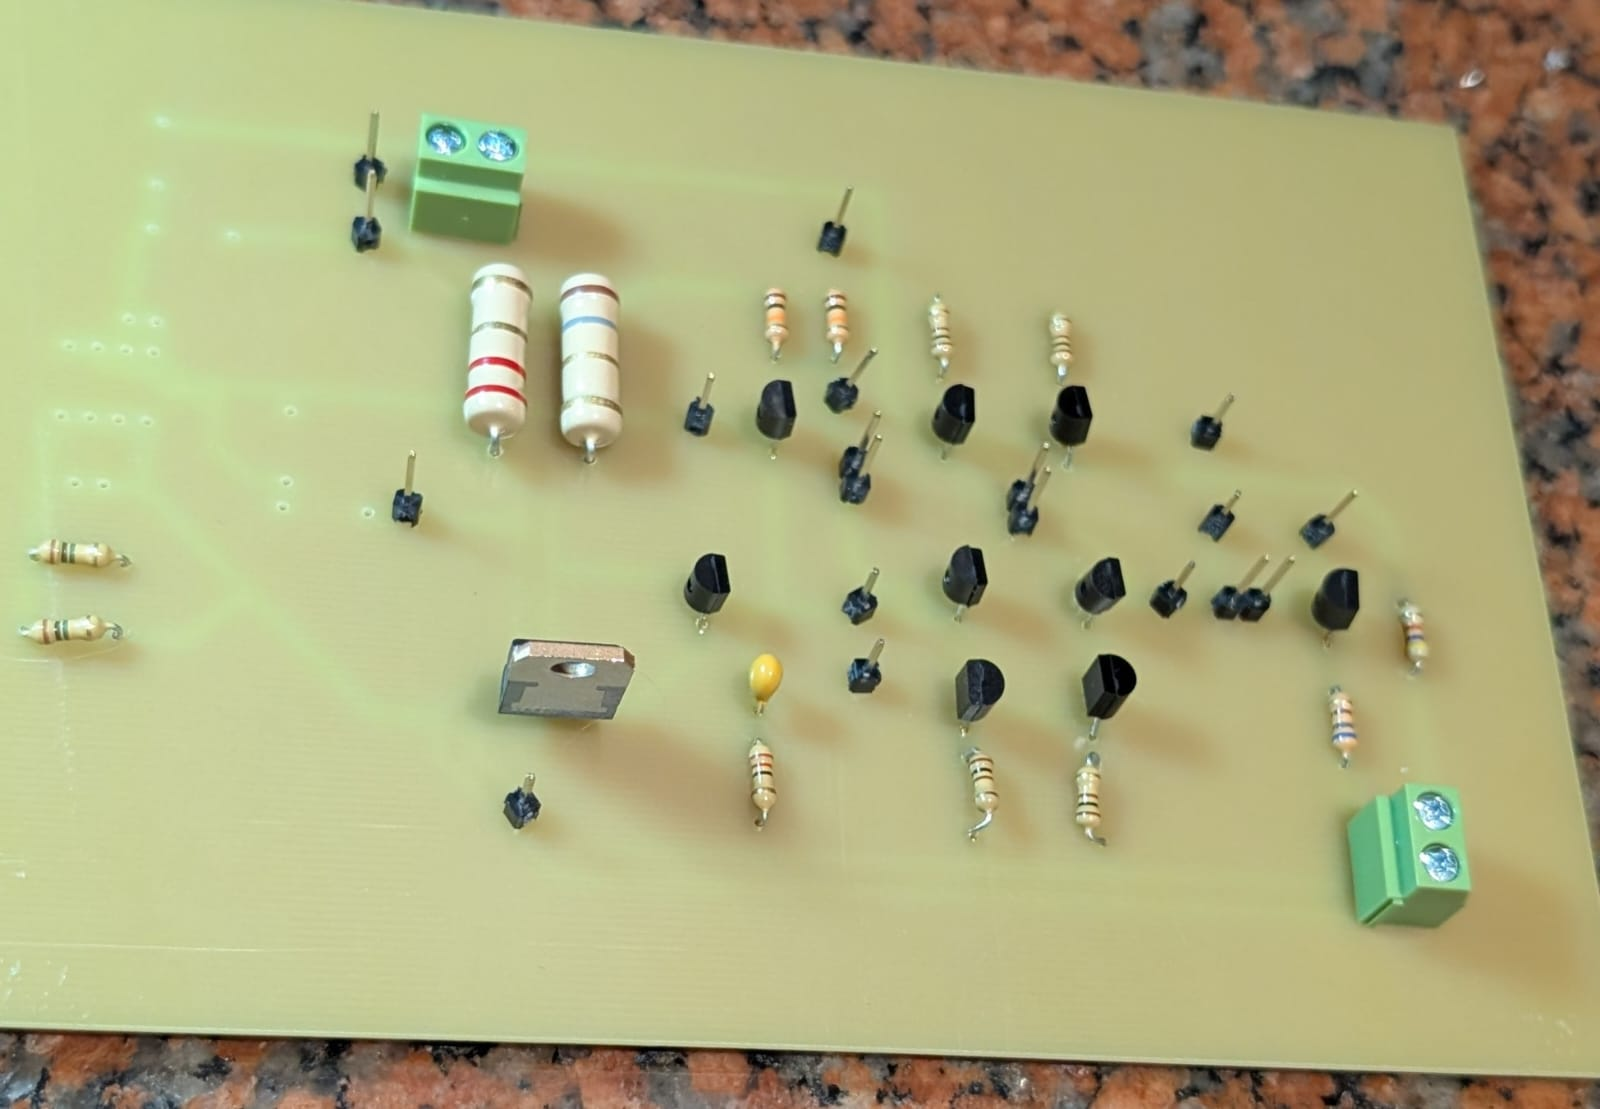
\includegraphics[width=0.65\textwidth]{img/soldado-lazo-tension.jpeg}
  \caption{Soldado correspondiente al lazo de tensión durante el proceso de montaje del PCB.}
  \label{fig:soldado-lazo-tension}
\end{figure}


\subsection{Lazo de Corriente}

Una vez verificado el correcto funcionamiento del lazo de regulación de tensión, se integró el amplificador operacional LM358 junto con la red de sensado correspondiente a la protección \textit{foldback}. Durante esta etapa se realizaron verificaciones funcionales sobre el lazo de corriente y el comportamiento general del sistema ante distintas condiciones de carga. En la Figura \ref{fig:soldado-lazo-corriente} se observa el resultado de la placa con todos los componentes soldados.

\begin{figure}[H]
  \centering
  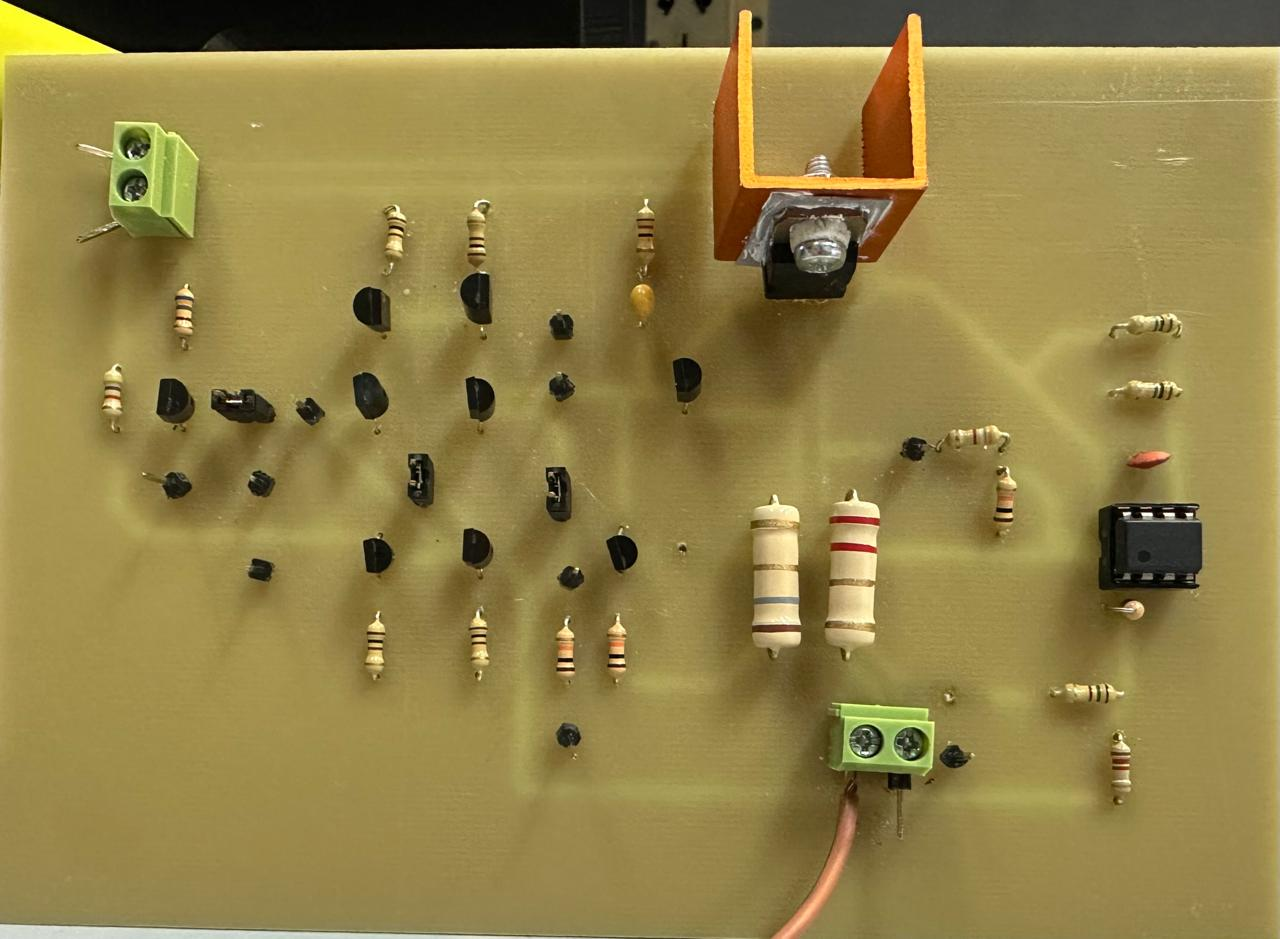
\includegraphics[width=0.65\textwidth]{img/soldado-lazo-corriente.jpeg}
  \caption{Soldado correspondiente al lazo de corriente durante el proceso de montaje del PCB.}
  \label{fig:soldado-lazo-corriente}
\end{figure}

\subsection{Contingencias de montaje}

Durante la implementación física, se identificaron inconvenientes de montaje y de \textit{layout} que condicionaron el proceso de armado y la depuración inicial del prototipo:

\begin{itemize}
    \item \textbf{Subdimensionamiento de pistas:} El ancho de varias pistas de señal resultó demasiado pequeño para un prototipo sometido a múltiples instancias de soldado y retrabajo manual. Esto redujo la superficie efectiva de cobre disponible, dificultó las tareas de montaje y aumentó la fragilidad mecánica de distintos nodos del circuito.
    
    \item \textbf{Desprendimiento de pads y deterioro del cobre:} La manipulación reiterada de la placa durante el proceso de depuración provocó el levantamiento de varias pistas y \textit{pads}, particularmente en zonas sometidas a retrabajo térmico frecuente. En algunos casos, ciertos terminales quedaron prácticamente sin superficie de cobre utilizable, dificultando significativamente la restauración de conexiones confiables. Para recuperar la continuidad eléctrica, fue necesario implementar puentes mediante conductores externos soldados directamente a los terminales de los componentes.
    
    \item \textbf{Falsos contactos durante la depuración:} La presencia de pistas debilitadas y conexiones mecánicamente inestables generó comportamientos erráticos durante las primeras pruebas del sistema. Si bien se realizaron verificaciones sistemáticas de continuidad, la reducida dimensión de algunas pistas dificultó la detección inmediata de falsos contactos y conexiones intermitentes. 
\end{itemize}

Estas dificultades evidenciaron que, para futuras iteraciones del PCB, resulta conveniente adoptar criterios de diseño más conservadores, incrementando el ancho de pista y el tamaño de los \textit{pads} para mejorar la robustez mecánica del montaje y facilitar las tareas de validación experimental y depuración.

\section{Rediseño del lazo de corriente}

Las primeras mediciones experimentales mostraron que el lazo de corriente interfería con el funcionamiento normal del regulador incluso en condiciones donde la protección \textit{foldback} debía permanecer inactiva. En particular, se observó que la tensión de salida no lograba regular en el valor esperado, aun cuando el lazo de tensión operaba correctamente de manera aislada.

A partir de estas observaciones, se decidió analizar el problema en una sección específica, ya que el comportamiento detectado no se debía únicamente a inconvenientes de montaje, sino también a limitaciones asociadas al diseño implementado para el lazo de corriente y a su interacción con la etapa de potencia.

\subsection{Problema detectado experimentalmente}

Durante los primeros ensayos se observó que el lazo de corriente interfería con el funcionamiento normal del regulador, aun en condiciones donde la protección \textit{foldback} debía permanecer inactiva. En particular, la tensión de salida quedaba limitada a aproximadamente $\SI{2.4}{\volt}$. Luego de varios experimentos, se detectó que la salida del amplificador operacional que activa el lazo de corriente era de $\SI{650}{\milli \volt}$ a pesar de que no hubiera carga, con lo cual el transistor de drenaje retiraba corriente de la base del quasidarlington. 

Repasando la hoja de datos del integrado se econtró la siguiente tabla. 

\begin{figure}[H]
  \centering
  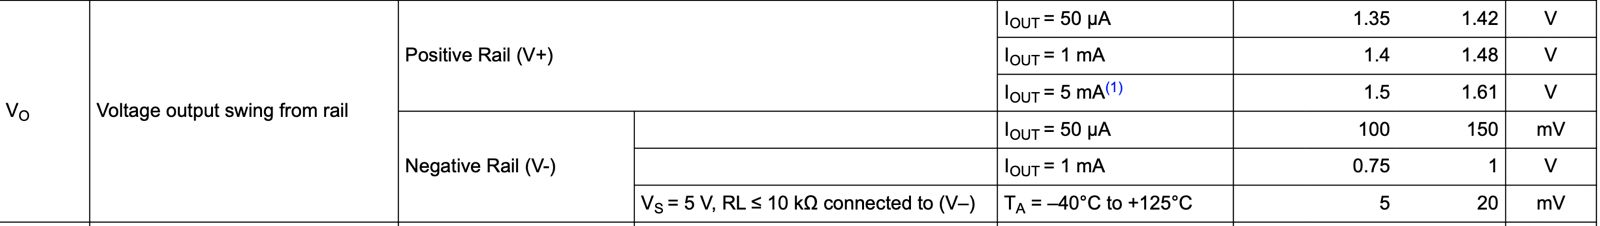
\includegraphics[width=0.9\textwidth]{img/tabla datasheet.jpeg}
  \caption{Especificaciones de la salida del operacional}
  \label{fig:tabla datasheet}
\end{figure}

En la misma, puede leerse que para una corriente de salida de $\SI{1}{\milli \ampere}$ la mínima tensión de salida posible es entre $\SI{0.75}{\volt}$ y $\SI{1}{\volt}$ mayor a la tensión del riel negativo. En este circuito, el riel negativo es $\SI{0}{\volt}$, por lo que este dato explica por qué el operacional polarizaba al transistor de drenaje de forma incorrecta. De esta forma, el error en el diseño original fue no incluir resistores entre la salida del amplificador y la base del TBJ que limitaran la corriente de salida del primero.


Por último, se simuló la etapa del operacional aislada del resto del circuito, y se encontró que la salida del mismo rondaba los $\SI{4}{\volt}$. De esta forma, es el TBJ el que fuerza a que la salida sea de $\SI{0.65}{\volt}$, lo que supone una demanda demasiado grande para el operacional.

\subsection{Modificación implementada}

Con el objetivo de estabilizar el estado de corte del transistor y reducir la carga impuesta sobre la salida del LM358, se incorporó una resistencia de \SI{1}{\kilo\ohm} entre la base del transistor de \textit{foldback} y masa. Este resistor actúa como un resistor de \textit{pull-down}, disminuyendo la tensión del nodo y dándole a la corriente un camino adicional para llegar a masa. 

Cabe mencionar que en el futuro se incluirá también un resistor de $\SI{3.9}{\kilo \Omega}$ para formar un divisor resistivo con el resistor ya mencionado y permitir así que la tensión de salida del operacional no sea forzada a $\SI{0.65}{\volt}$. Sin embargo, en las mediciones hechas en este informe no se la pudo incluir por falta de tiempo. 

\subsection{Validación posterior al cambio}
Una vez incorporada la modificación, se repitieron las mediciones relevantes para verificar el comportamiento del lazo de corriente bajo distintas condiciones de carga. A diferencia de las primeras pruebas, el circuito pasó a exhibir una respuesta consistente con la prevista durante el diseño, observándose un funcionamiento estable tanto del lazo de tensión como de la protección \textit{foldback}.

La incorporación de la resistencia de \textit{pull-down} permitió evitar activaciones espurias del transistor asociado al lazo de corriente y redujo la carga impuesta sobre la salida del LM358. De esta manera, la validación experimental posterior confirmó que el comportamiento anómalo observado inicialmente estaba asociado principalmente al criterio de conexión adoptado en el diseño original y no únicamente a problemas de montaje.

\section{Mediciones}

En esta sección se detallan las mediciones efectuadas. En las Figuras \ref{fig:banco-medicion-1} y \ref{fig:banco-medicion-2} se muestran los bancos de trabajo utilizados para realizar los ensayos experimentales.

\begin{figure}[H]
  \centering
  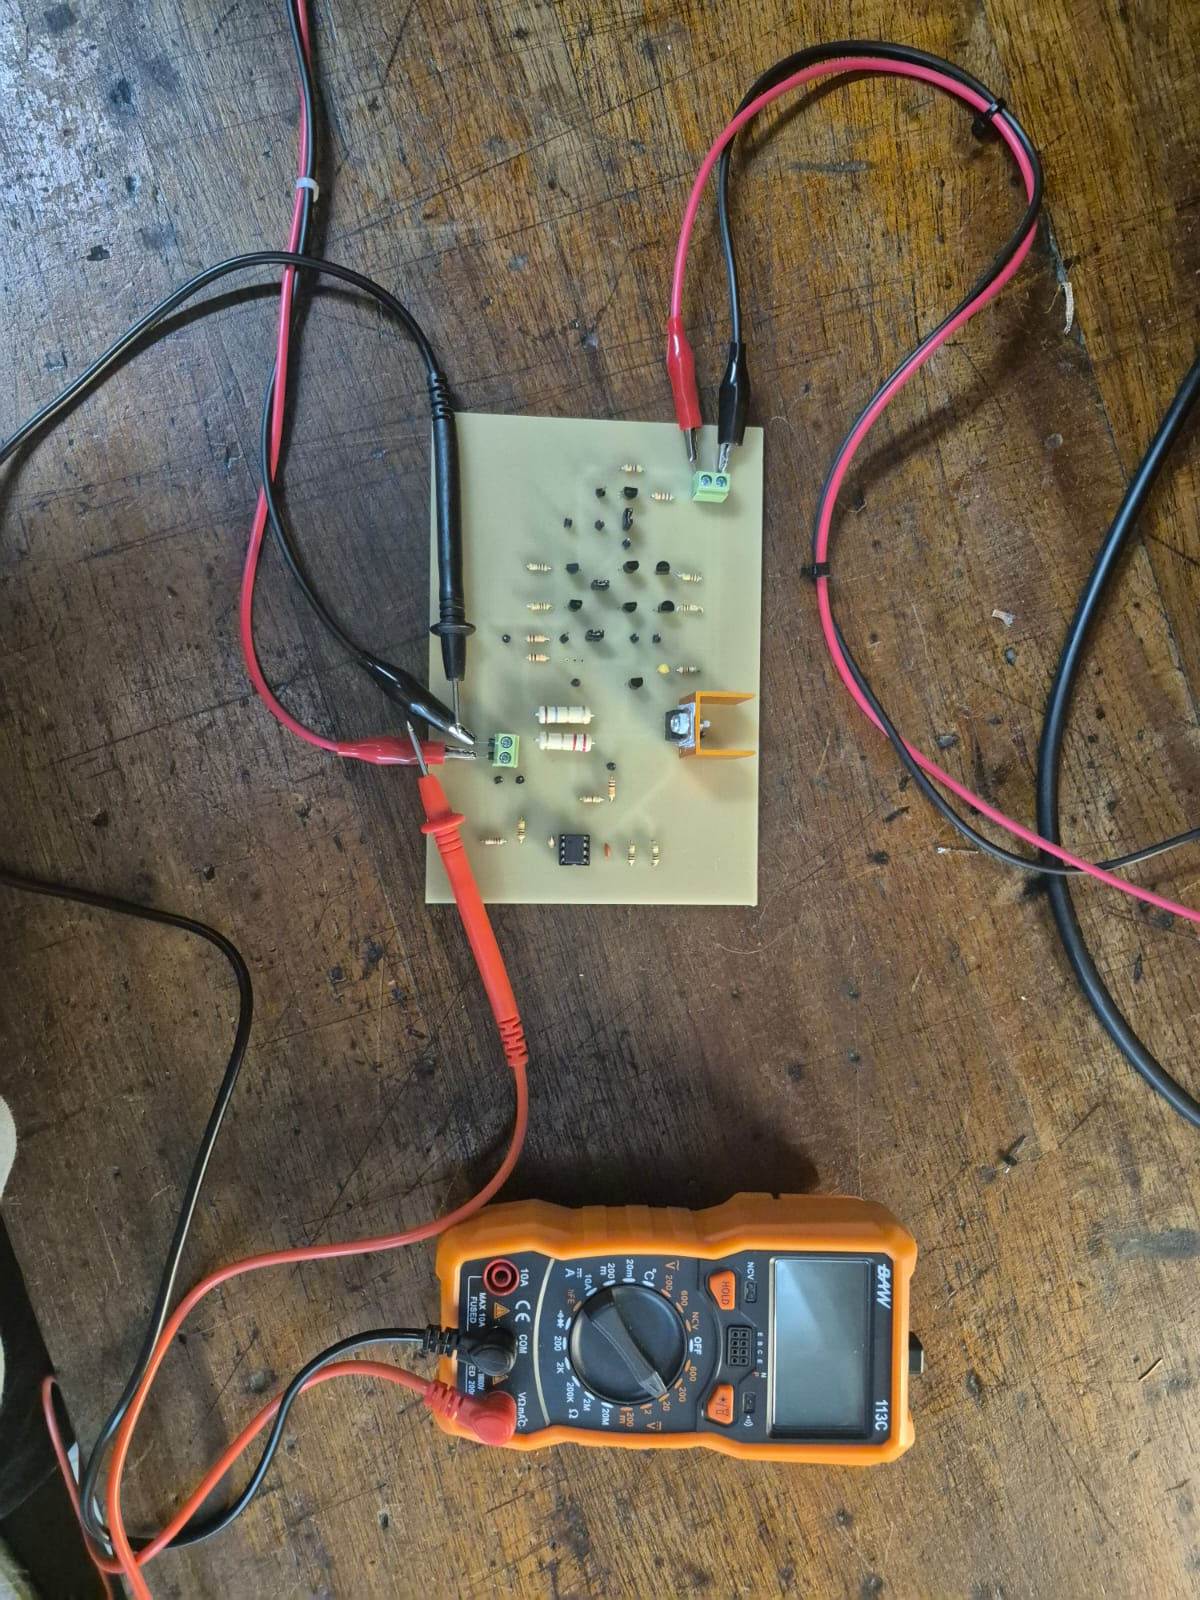
\includegraphics[angle=90,width=0.75\textwidth]{img/banco-medicion-1.jpeg}
  \caption{Primer banco de medición utilizado durante la validación experimental del regulador.}
  \label{fig:banco-medicion-1}
\end{figure}

\begin{figure}[H]
  \centering
  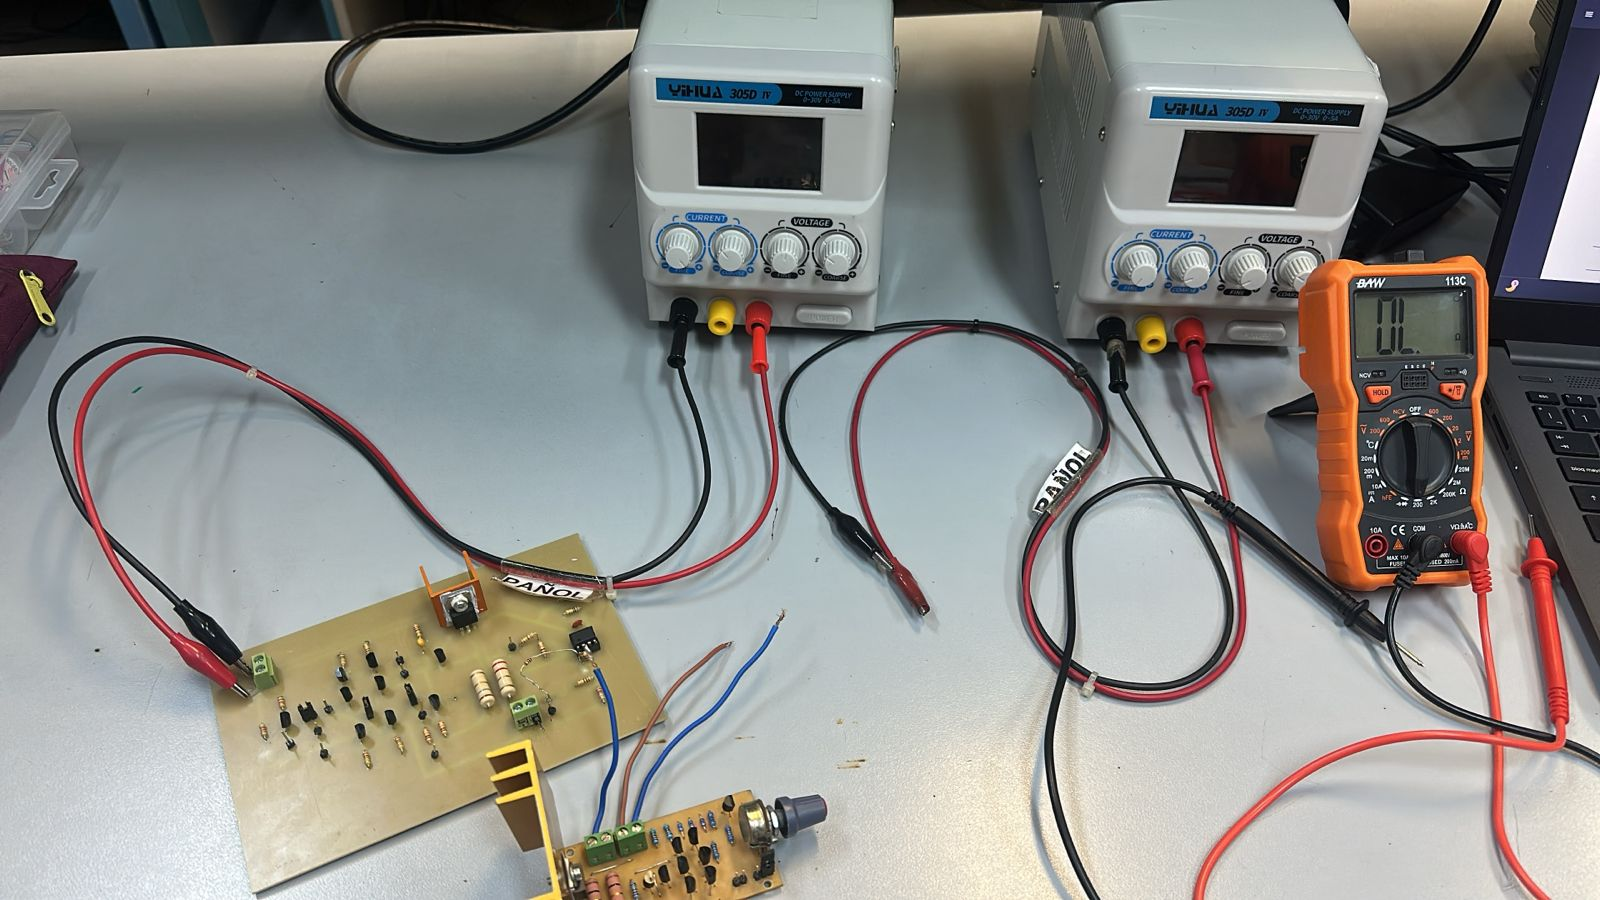
\includegraphics[width=0.75\textwidth]{img/banco-medicion-2.jpeg}
  \caption{Segundo banco de medición utilizado durante la validación experimental del regulador con carga electrónica.}
  \label{fig:banco-medicion-2}
\end{figure}

\subsection{Eficiencia}

Para una tensión de entrada de 9,5 V, una corriente de entrada de 182 mA, una tensión de salida de 5,01 V y una corriente de salida de 167 mA, dada por una carga estática de 30 $\Omega$, se registró una eficiencia del 48,39 \%. Este cálculo se hizo teniendo en cuenta las potencias de entrada y salida, como se muestra a continuación.

\[
\eta = \frac{P_o}{P_i} = \frac{V_o I_o}{V_i I_i} = 48,39 \,\text{\%}
\]

De este modo, se puede observar que la eficiencia conseguida depende de la corriente de salida (a tensión de salida constante) y de la tensión de entrada. En las Figuras \ref{fig:eta1} y \ref{fig:eta2} se muestra la eficiencia en función de la tensión de entrada a una corriente de salida constante de 1 A y en función de la corriente de salida a una tensión de entrada constante de 9,5 V, respectivamente.

\begin{figure}[H]
  \centering
  \begin{minipage}[t]{0.48\textwidth}
    \centering
    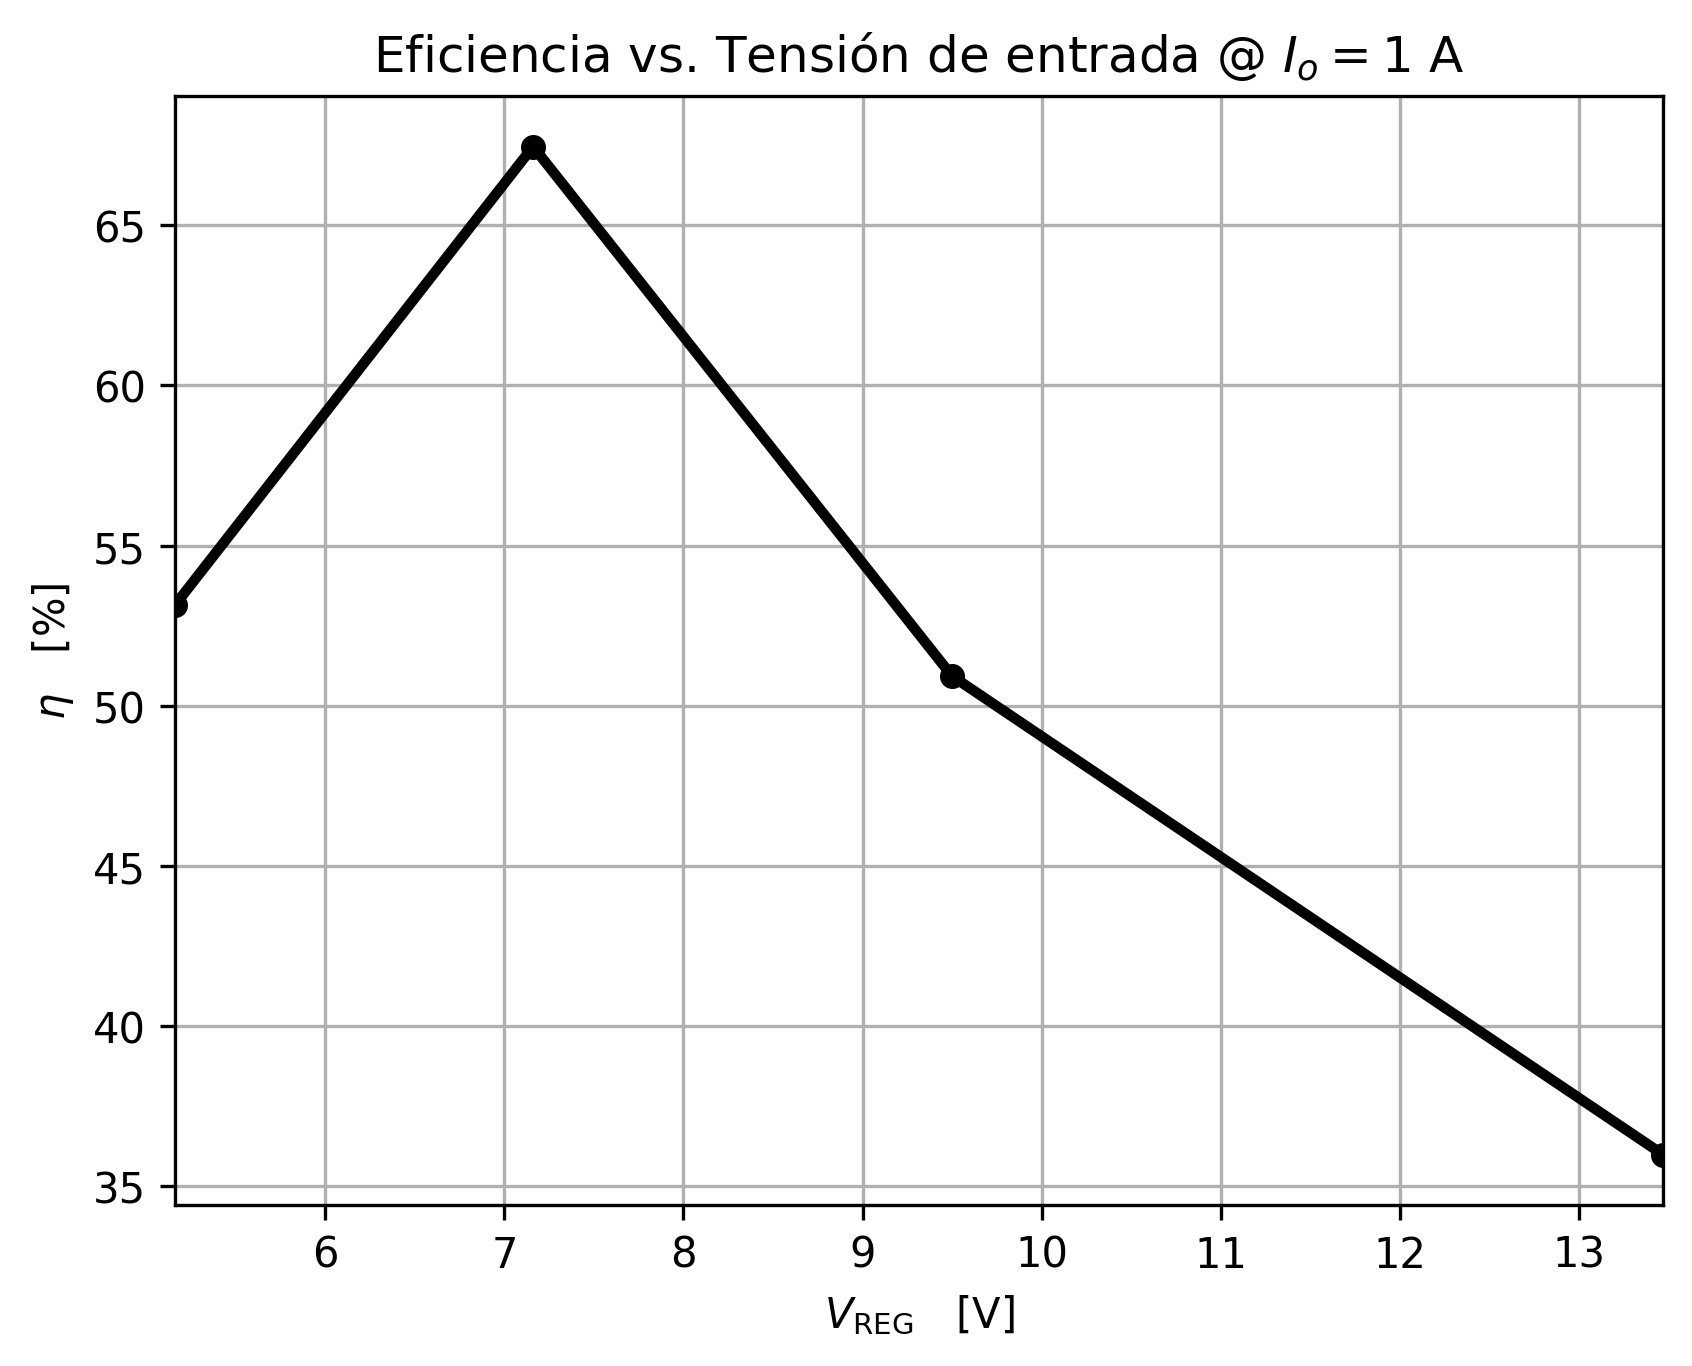
\includegraphics[width=\textwidth]{img/eficiencia_vs_vreg.png}
    \caption{Eficiencia del circuito en función de la tensión de entrada para una corriente de salida de 1 A.}
    \label{fig:eta1}
  \end{minipage}
  \hfill
  \begin{minipage}[t]{0.48\textwidth}
    \centering
    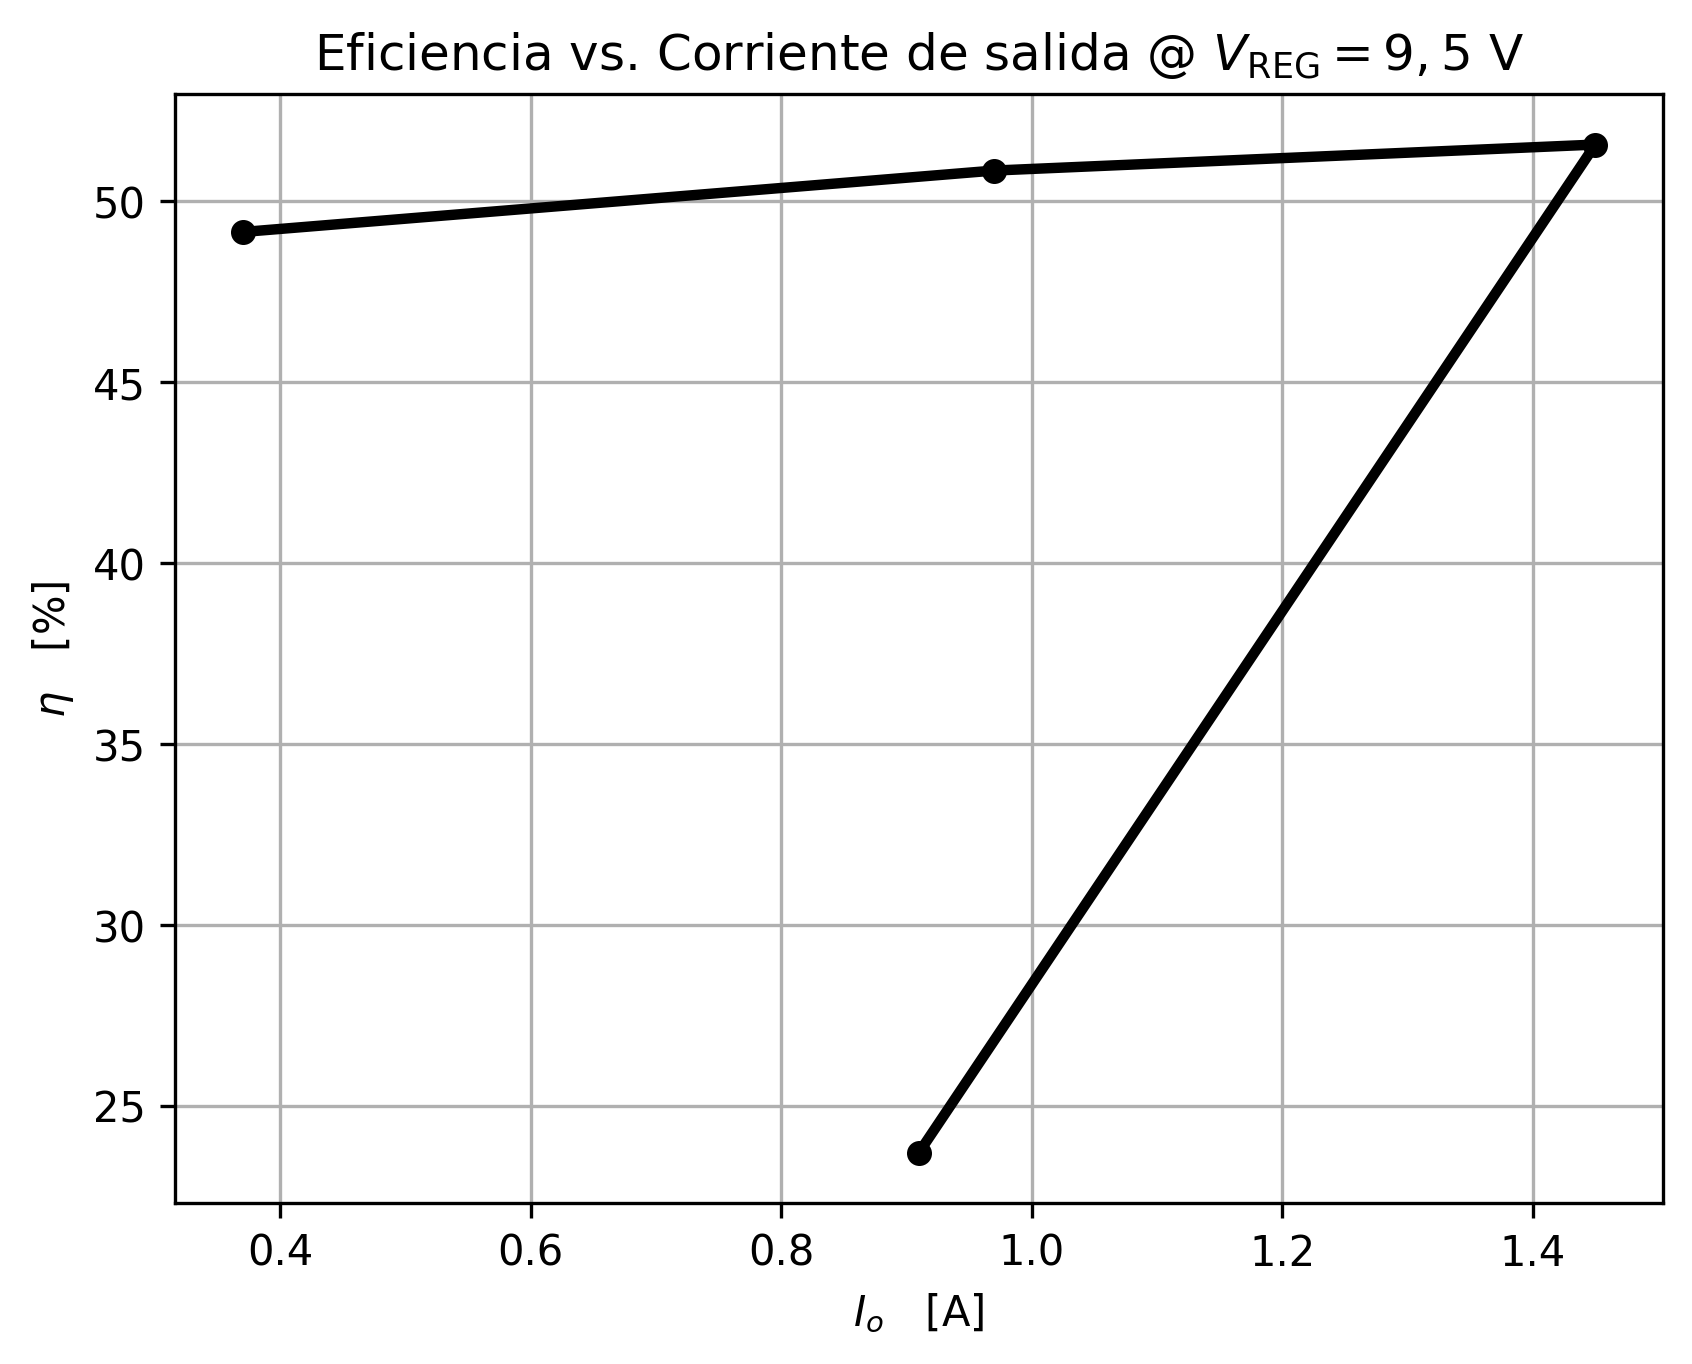
\includegraphics[width=\textwidth]{img/eficiencia_vs_io.png}
    \caption{Eficiencia del circuito en función de la corriente de salida para una tensión de entrada de 9,5 V.}
    \label{fig:eta2}
  \end{minipage}
\end{figure}

\subsection{Regulación de línea}

La regulación de línea se obtuvo midiendo con una carga estática de 50 $\Omega$ que fija una corriente de salida de 100 mA y variando la tensión regulada que ingresa al LDO. El resultado fue 11,86 mV/V: un 41,02 \% mayor que el valor teórico ---probablemente atribuido a la escasez de mediciones---.
La curva resultante de la medición se muestra en la Figura \ref{fig:reg_lin}. 

\begin{figure}[H]
  \centering
  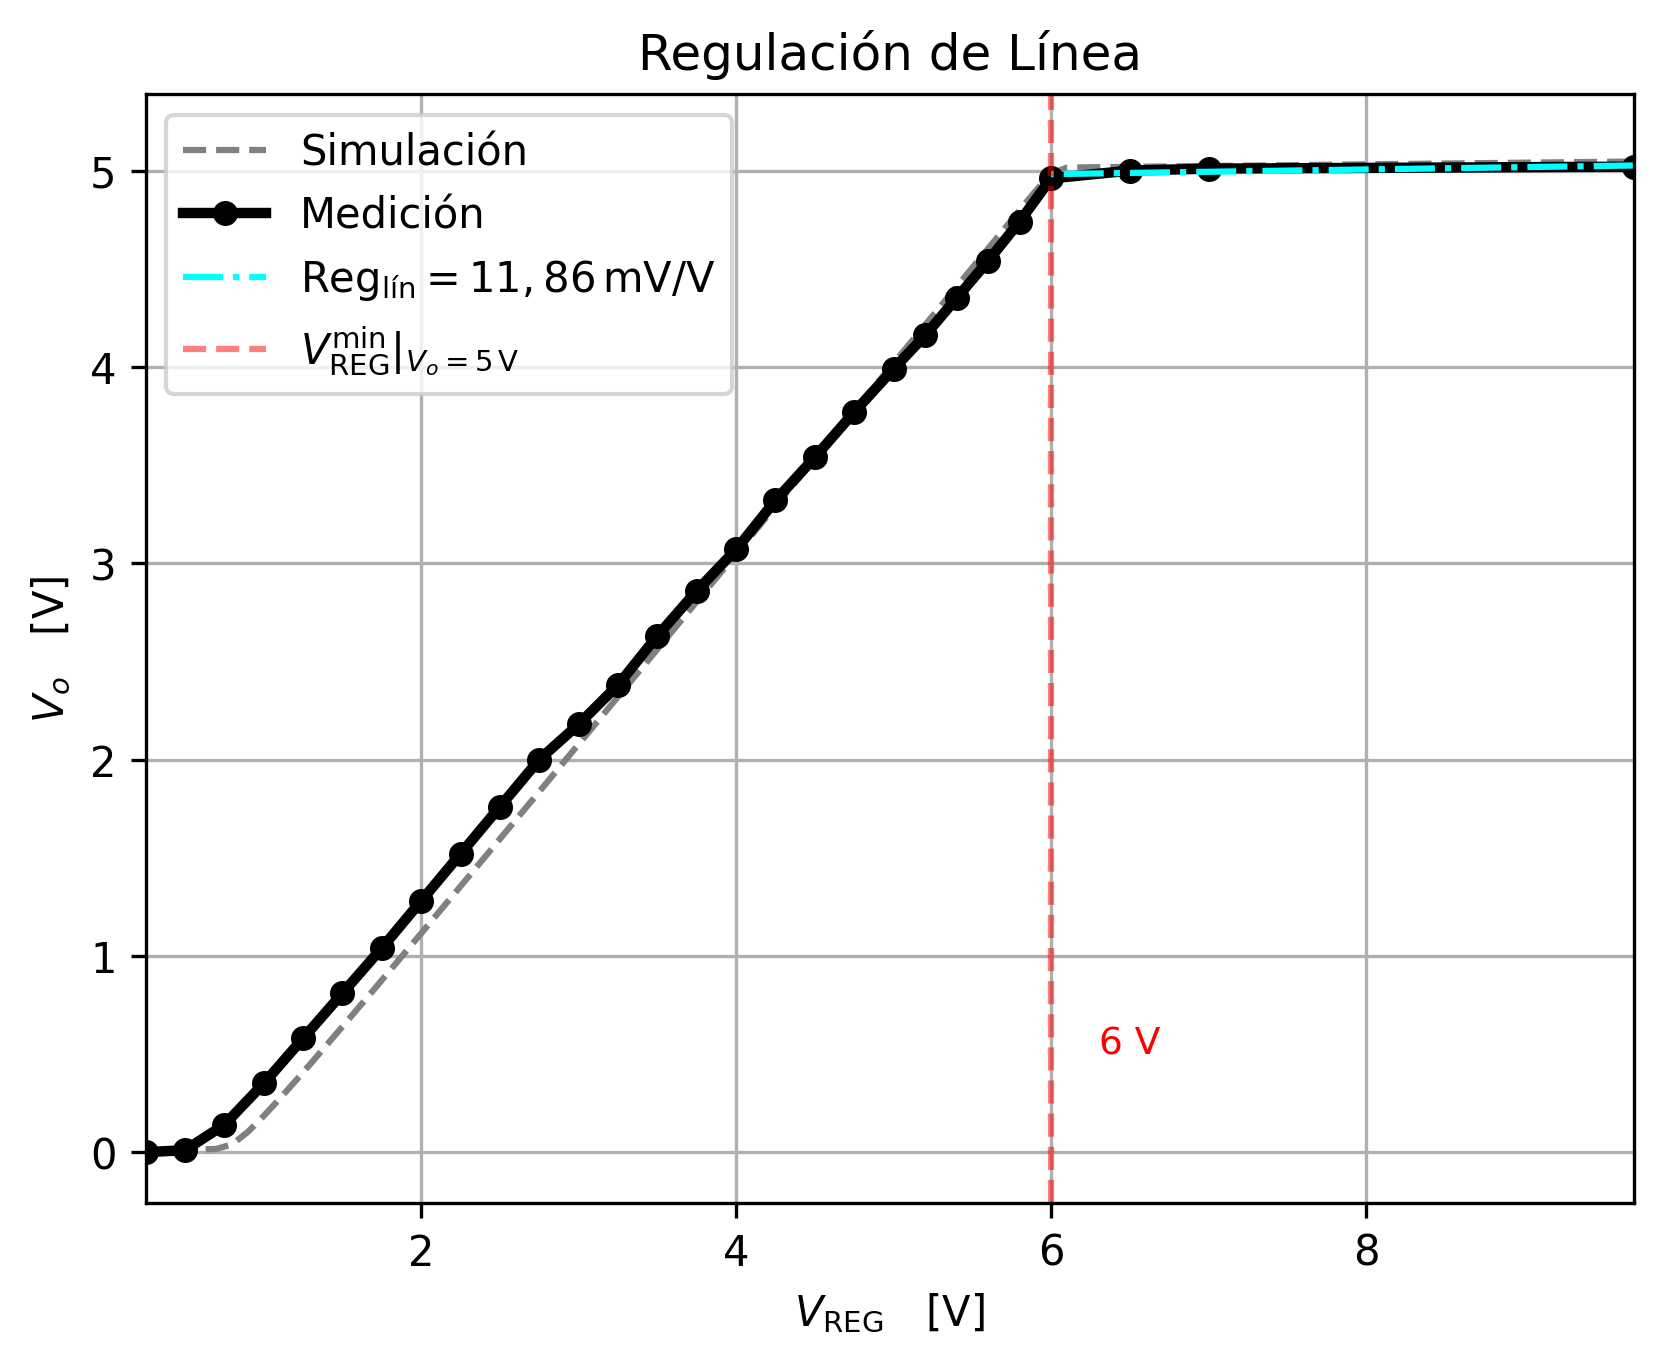
\includegraphics[width=0.8\textwidth]{img/reg_lin.png}
  \caption{Regulación de línea medida y simulada.}
  \label{fig:reg_lin}
\end{figure}

Nótese que $V_\text{REG}^\text{min}\Big|_{V_o = 5\,\text{V}} = 6\,\text{V}$, por lo que se obtiene una tensión de \textit{dropout} de

\[
V_\text{drop} = V_\text{REG}^\text{min}\Big|_{V_o = 5\,\text{V}} - V_o = 1\,\text{V},
\]

valor que coincide exactamente con el teórico.

\subsection{Regulación de carga}

En esta sección se detallan las mediciones correspondientes a la regulación de carga.

\subsubsection{Estática}

En la Figura \ref{fig:reg_car} se muestra la tensión de salida en función de la resistencia de carga. Allí se observa que el rango de operación del lazo de tensión efectivamente es para cargas mayores a 3,33 $\Omega$.

\begin{figure}[H]
  \centering
  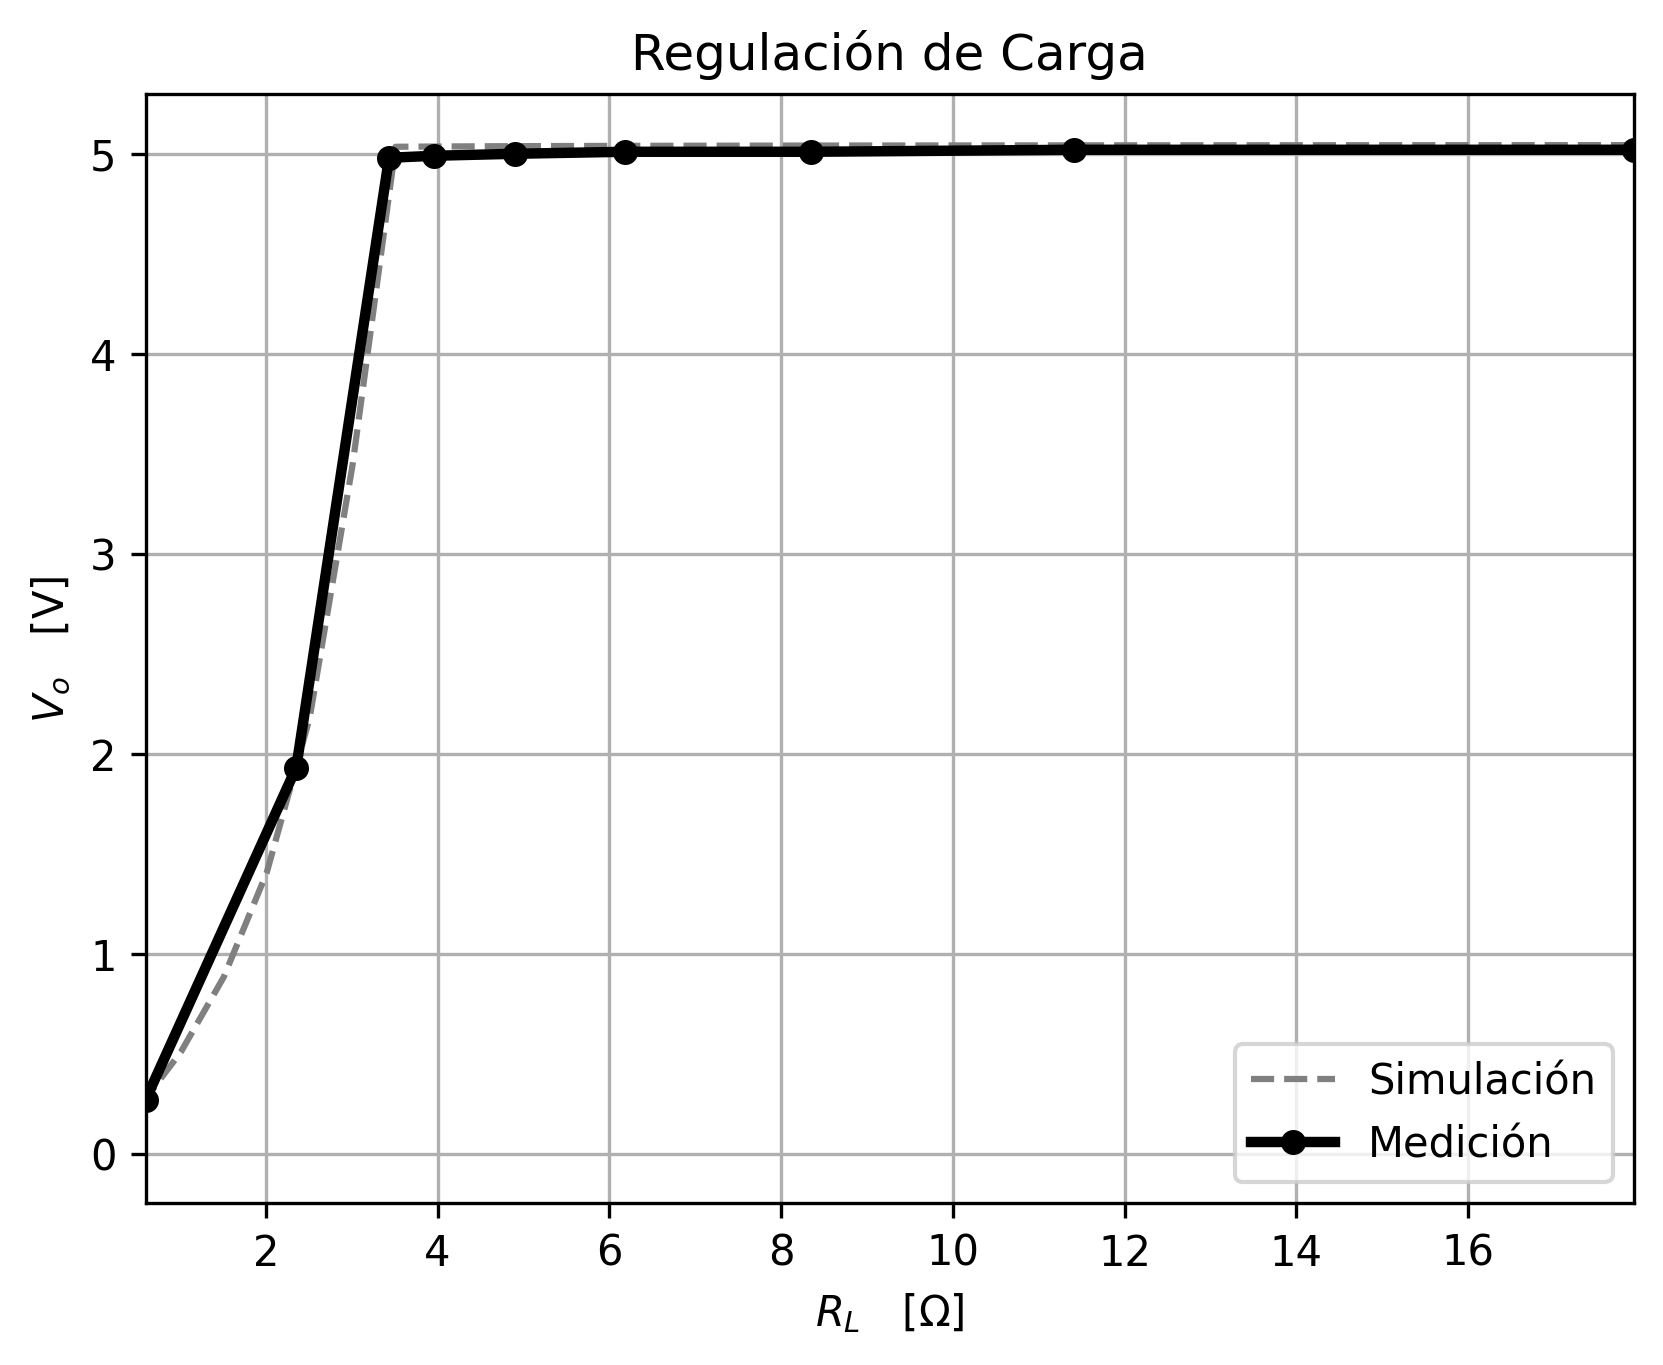
\includegraphics[width=0.75\textwidth]{img/reg_car.png}
  \caption{Regulación de carga medida y simulada.}
  \label{fig:reg_car}
\end{figure}

El valor de la regulación de carga se obtiene de la curva del \textit{foldback}, mostrada en la Figura \ref{fig:foldback}, el cual es de 28,81 m$\Omega$: un 75,46 \% mayor que el valor teórico, aunque aún muy aceptable. Se observa que la corriente límite es de 1,45 A y que la corriente de \textit{foldback} es de 450 mA.

\begin{figure}[H]
  \centering
  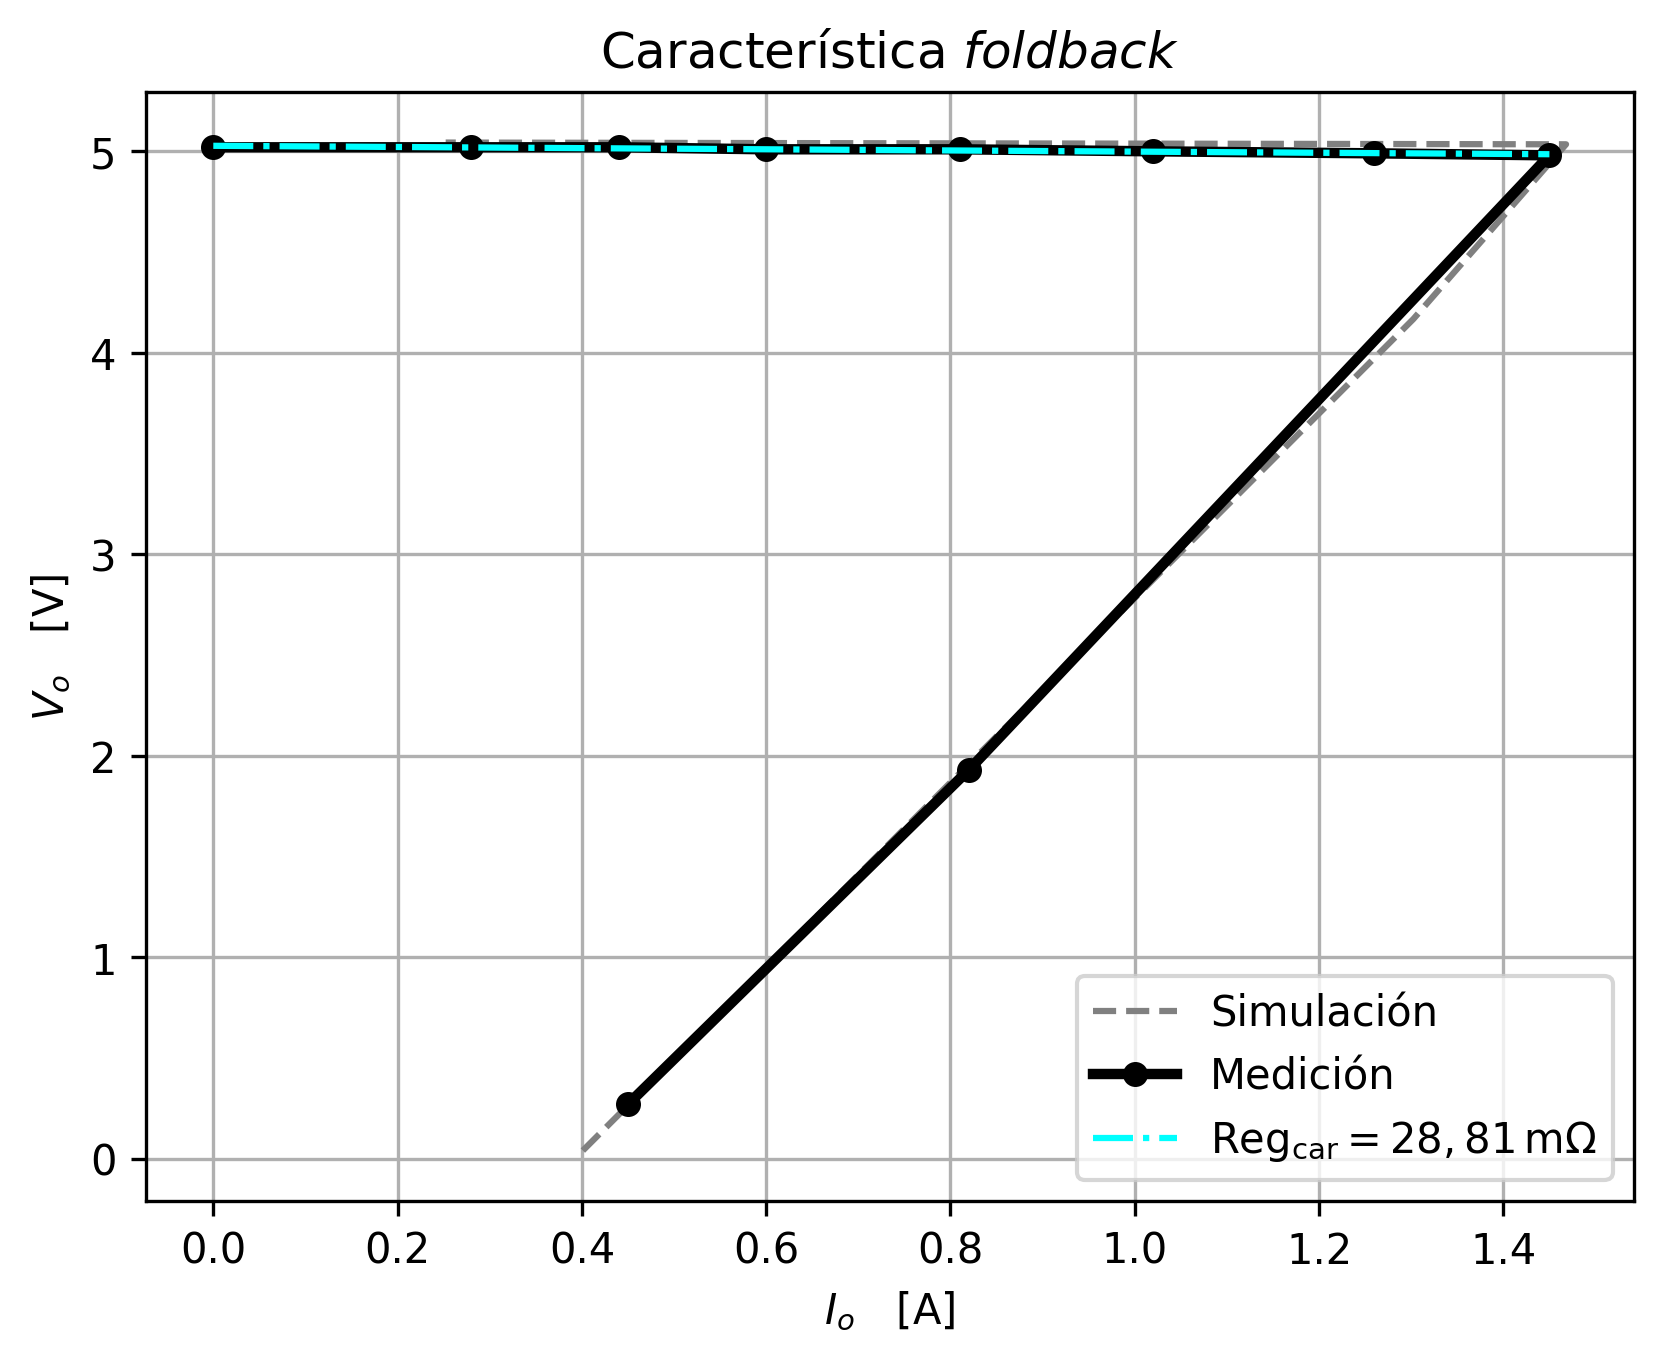
\includegraphics[width=0.75\textwidth]{img/foldback.png}
  \caption{Curva del \textit{foldback}.}
  \label{fig:foldback}
\end{figure}

\subsubsection{Dinámica}

La regulación de carga dinámica evalúa la capacidad del regulador para mantener estable la tensión de salida frente a variaciones rápidas de corriente demandada por la carga. Esta medición permite analizar la respuesta transitoria del sistema y verificar experimentalmente el comportamiento dinámico del lazo de control.

Para realizar el ensayo, se implementó una carga dinámica con un transistor MOSFET, modelo IRFZ46N. Sobre su compuerta se aplicó una señal cuadrada proveniente de un generador de funciones. Además, se conectó una resistencia de $\SI{33}{\Omega}$ al terminal source, mientras que el terminal drain se vinculó a la salida del regulador. De esta manera, la señal aplicada al MOSFET permitía conectar y desconectar periódicamente la carga, generando escalones de corriente sobre la salida del regulador. La respuesta temporal de la tensión de salida se observó mediante osciloscopio, analizando el comportamiento transitorio del sistema frente a dichas perturbaciones dinámicas. Con el banco de medición de la Figura \ref{fig:banco-carga-dinamica} se obtuvo la respuesta mostrada en la Figura \ref{fig:carga-dinamica}.


\begin{figure}[H]
  \centering
  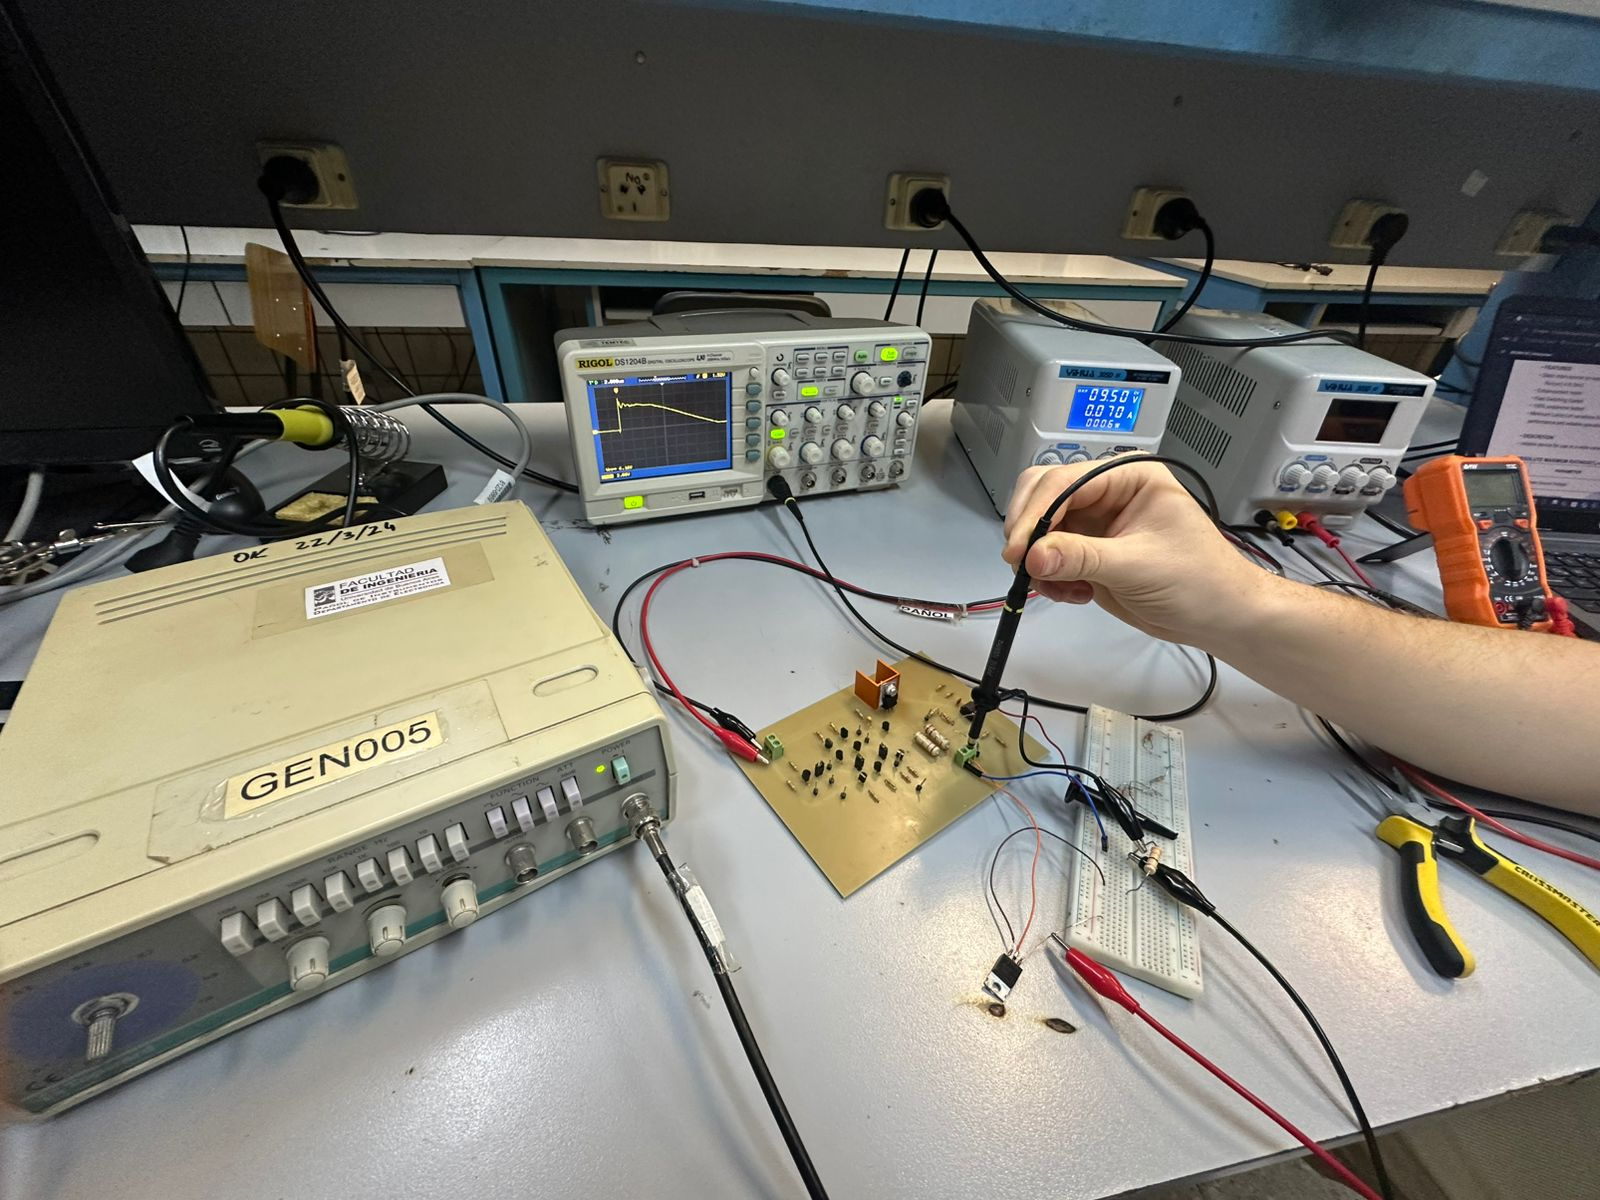
\includegraphics[width=0.8\textwidth]{img/banco carga dinamica.jpg}
  \caption{Banco de medición para la regulación de carga dinámica}
  \label{fig:banco-carga-dinamica}
  
\end{figure}

\begin{figure}[H]
  \centering
  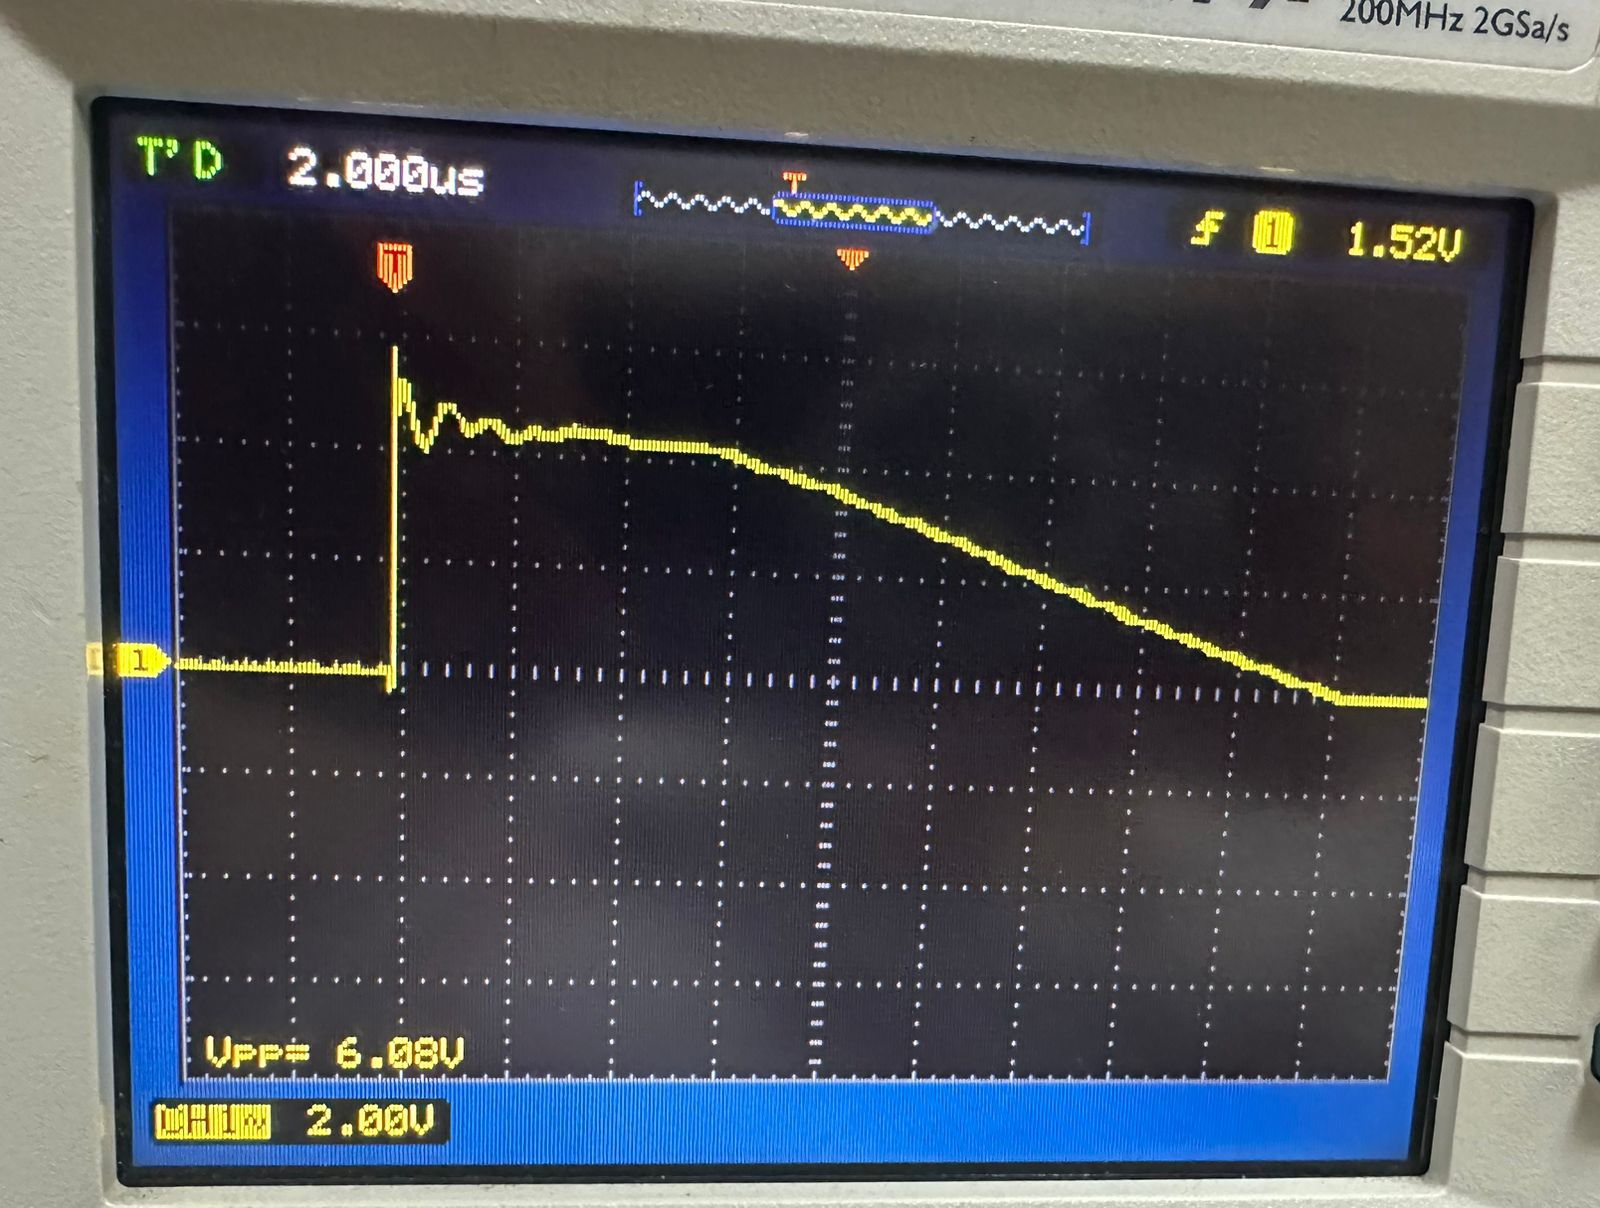
\includegraphics[width=0.8\textwidth]{img/Carga dinamica.jpg}
  \caption{Regulación de carga dinámica}
  \label{fig:carga-dinamica}
  
\end{figure}

\subsection{Respuestas a señales cuadradas}

\subsubsection{Lazo de tensión}

Con el objetivo de validar experimentalmente la compensación implementada durante la etapa de diseño, se evaluó la respuesta temporal del lazo de tensión frente a una perturbación aplicada sobre la referencia del regulador.

Para ello, se superpuso una señal de aproximadamente $\SI{50}{\milli\volt_{pp}}$ sobre la tensión de referencia, observándose la evolución temporal de la tensión de salida mediante osciloscopio. Con el objetivo de visualizar únicamente la respuesta dinámica del regulador frente a la perturbación introducida, las mediciones se realizaron utilizando acoplamiento AC en el osciloscopio, desacoplando así la componente continua de la salida.

Esta medición permitió analizar la capacidad del lazo para regular frente a pequeñas perturbaciones y verificar experimentalmente la estabilidad prevista durante las simulaciones.  

Como se puede observar en la Figura \ref{fig:respuesta-escalon-tension}, las mediciones obtenidas mostraron una respuesta estable, sin evidencia de oscilaciones sostenidas ni comportamientos inestables, validando así la estrategia de compensación adoptada para el lazo de tensión.

\begin{figure}[H]
  \centering
  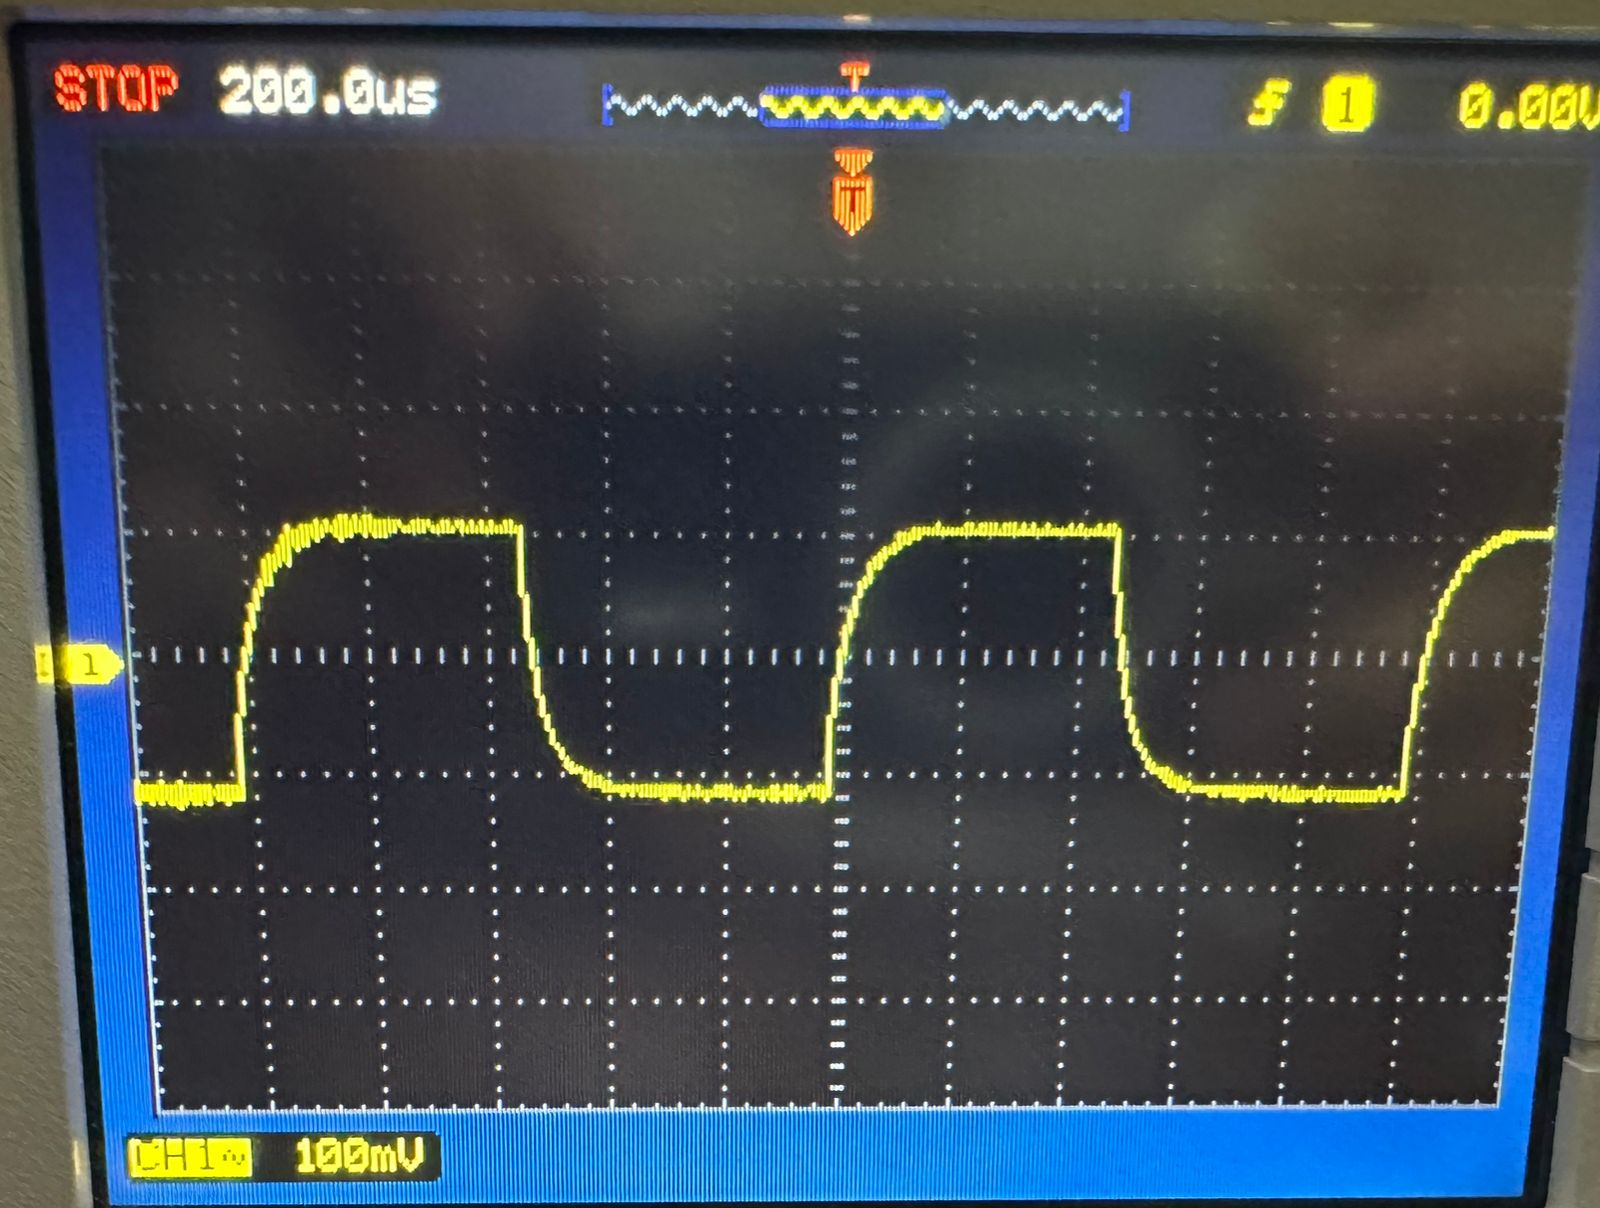
\includegraphics[width=0.5\textwidth]{img/respuesta-escalon-tension.jpeg}
  \caption{Respuesta del lazo de tensión a un escalón de $\SI{50}{\milli\volt_{pp}}$ con la continua desacoplada.}
  \label{fig:respuesta-escalon-tension}
\end{figure}


\subsubsection{Validación experimental de la respuesta en frecuencia}

A partir de la compensación realizada durante el \textit{checkpoint} 2, se obtuvo para el lazo de tensión una frecuencia de corte aproximada de $\SI{100}{\hertz}$. Con el objetivo de validar experimentalmente este comportamiento dinámico, se realizaron ensayos temporales y espectrales sobre la respuesta del regulador.

Para ello, se inyectó mediante un generador de funciones una señal cuadrada sobre la entrada no inversora correspondiente a la referencia del regulador. La señal aplicada tuvo una amplitud comprendida entre $0$ y $\SI{2.5}{\volt}$ y una frecuencia de $\SI{10}{\hertz}$.

La elección de esta frecuencia se realizó considerando que una señal cuadrada puede representarse como una suma de armónicos impares. Dado que el ancho de banda estimado del lazo era cercano a $\SI{100}{\hertz}$, se esperaba que los primeros armónicos de la señal aplicada atravesaran el sistema con escasa atenuación, reproduciendo adecuadamente la forma temporal de la onda a la salida.

Las Figuras \ref{fig:entrada-10Hz} y \ref{fig:salida-10Hz} muestran respectivamente la señal aplicada y la respuesta observada a la salida del regulador. Experimentalmente se verificó que la forma de onda de salida reproduce correctamente la excitación aplicada.

\begin{figure}[H]
  \centering
  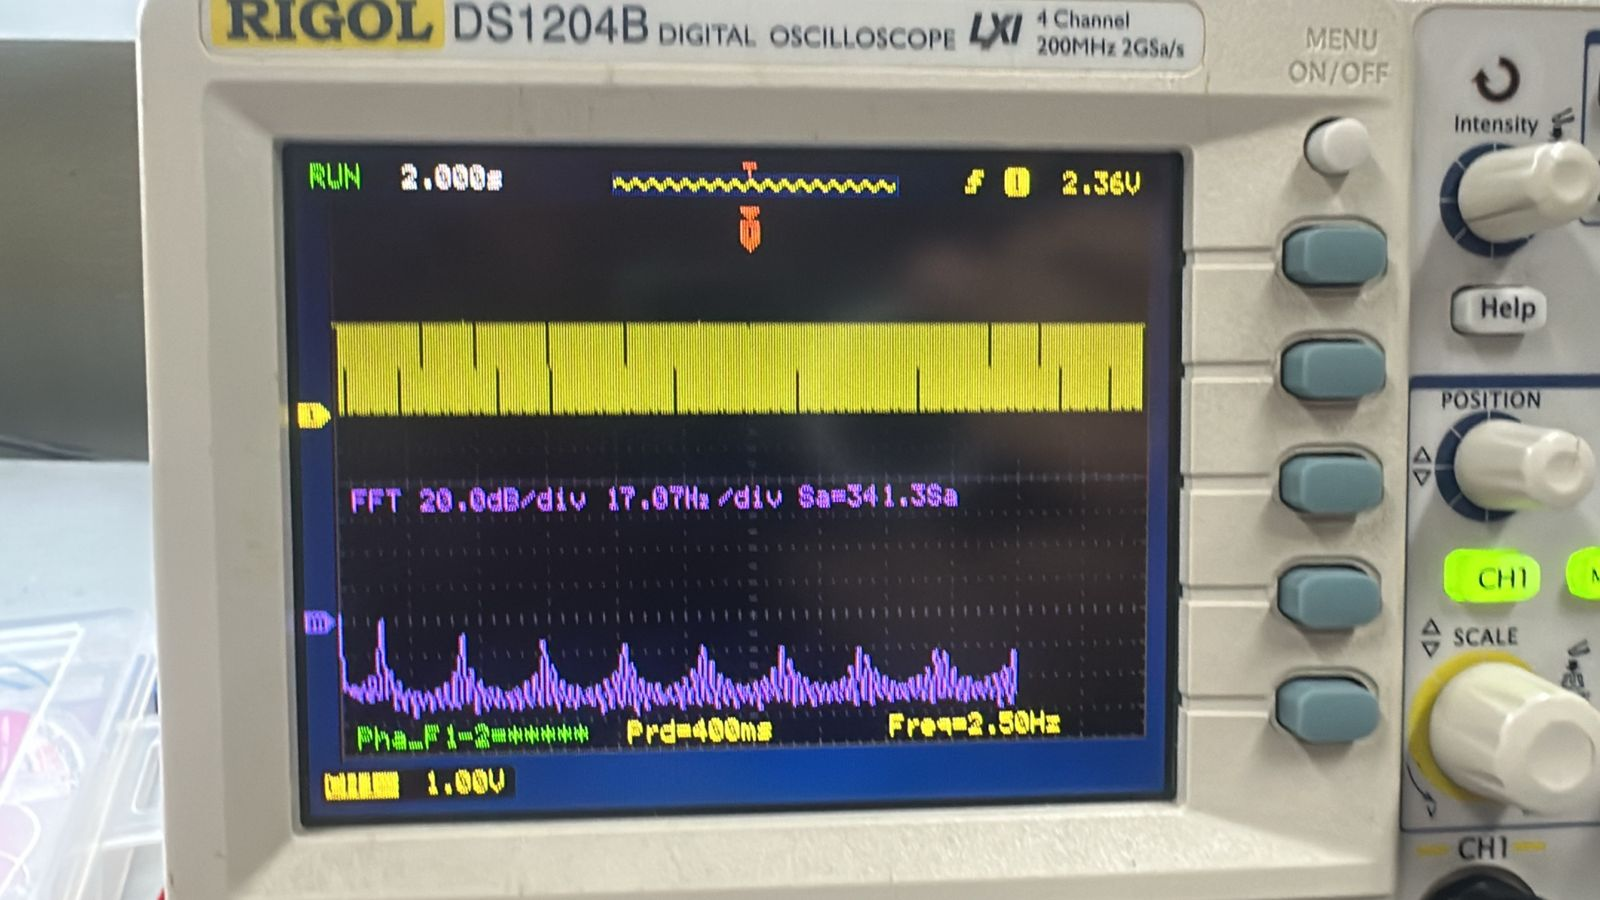
\includegraphics[width=0.5\textwidth]{img/entrada-10Hz.jpeg}
  \caption{Respuesta en tiempo y en frecuencia de una señal de entrada cuadrada de $\SI{10}{\hertz}$ en lugar de $V_\text{ref}$.}
  \label{fig:entrada-10Hz}
\end{figure}

\begin{figure}[H]
  \centering
  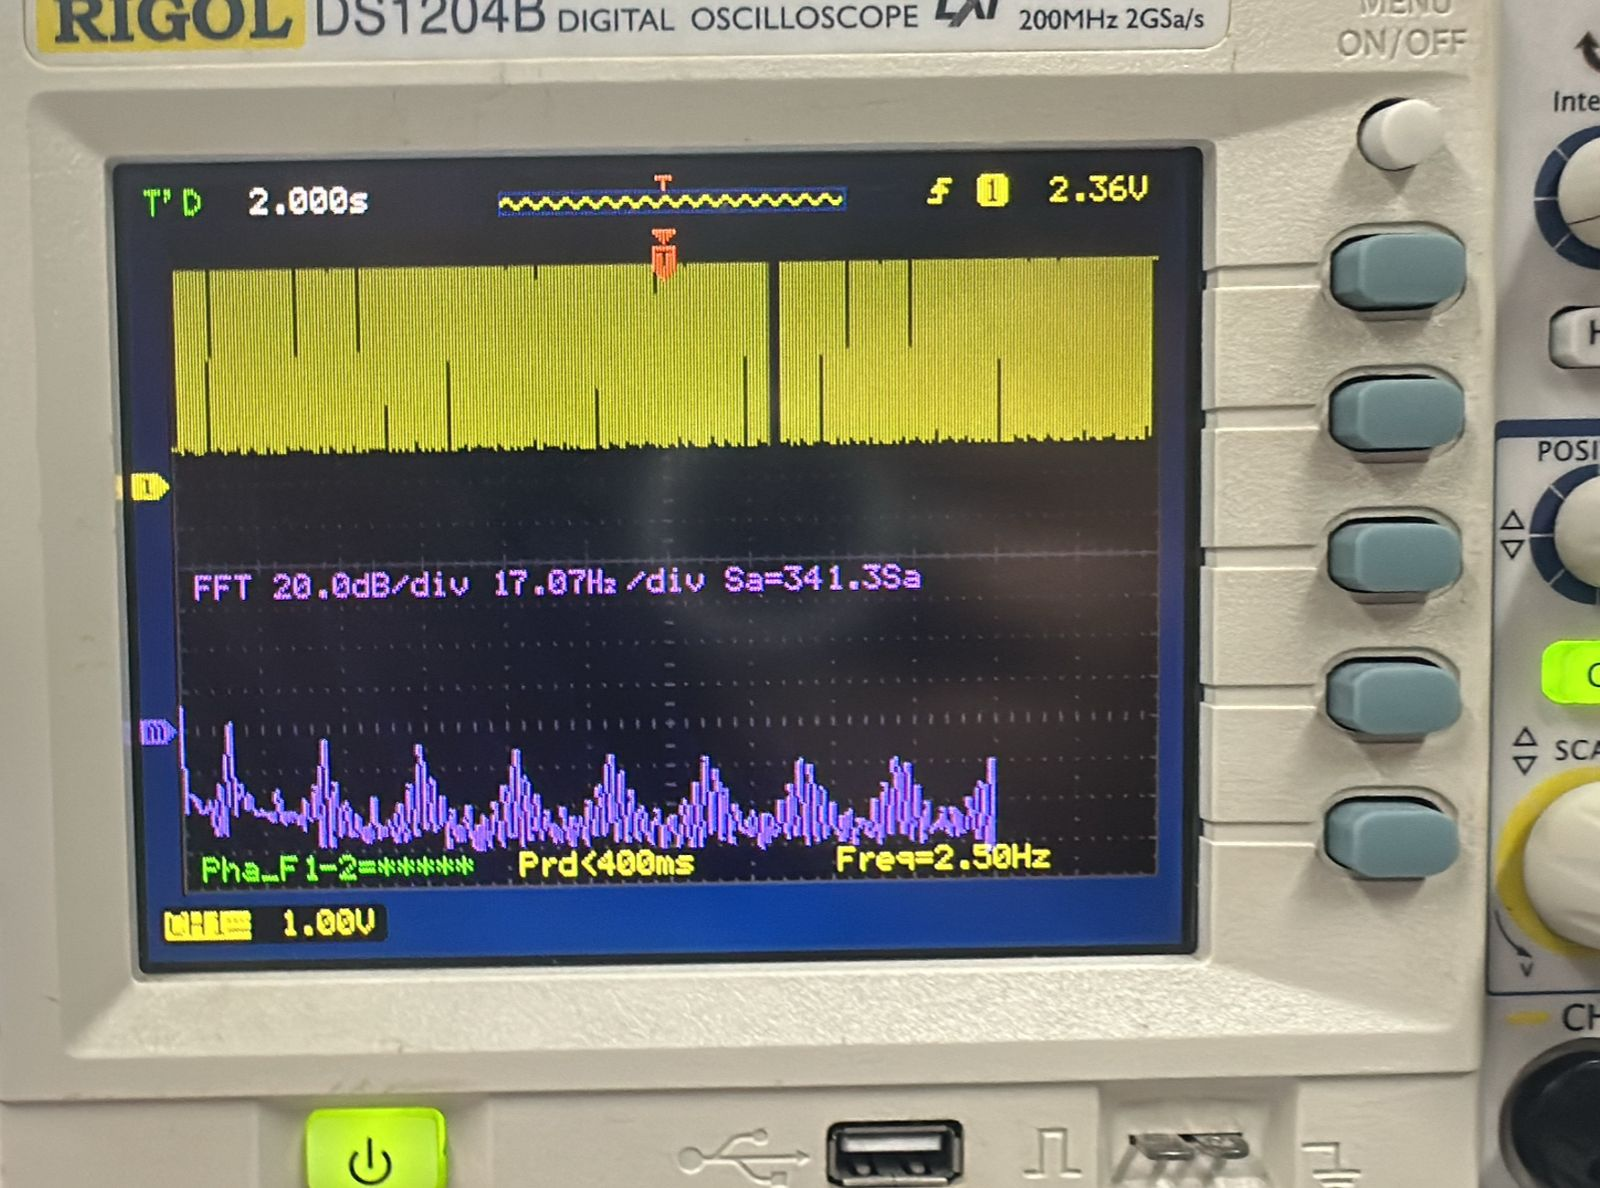
\includegraphics[width=0.5\textwidth]{img/salida-10Hz.jpeg}
  \caption{Respuesta en tiempo y en frecuencia de la señal de salida con una cuadrada de $\SI{10}{\hertz}$ aplicada en la entrada en lugar de $V_\text{ref}$.}
  \label{fig:salida-10Hz}
\end{figure}


Mediante la herramienta FFT del osciloscopio se observó que tanto en la entrada como en la salida se conservaban aproximadamente los primeros nueve armónicos de la señal, en concordancia con el comportamiento esperado para un sistema cuyo ancho de banda supera ampliamente la frecuencia fundamental utilizada en el ensayo.

Posteriormente, se repitió el ensayo utilizando una señal cuadrada de $\SI{100}{\hertz}$, frecuencia cercana al ancho de banda simulado para el lazo de tensión compensado durante el diseño.

A diferencia del caso anterior, la señal observada a la salida presentó una deformación apreciable respecto de la excitación original (esto se observa en las figuras \ref{fig:entrada-100Hz} y \ref{fig:salida-100Hz}). El análisis espectral mediante FFT mostró además la aparición de armónicos pares, inexistentes en la señal cuadrada ideal aplicada a la entrada.

\begin{figure}[H]
  \centering
  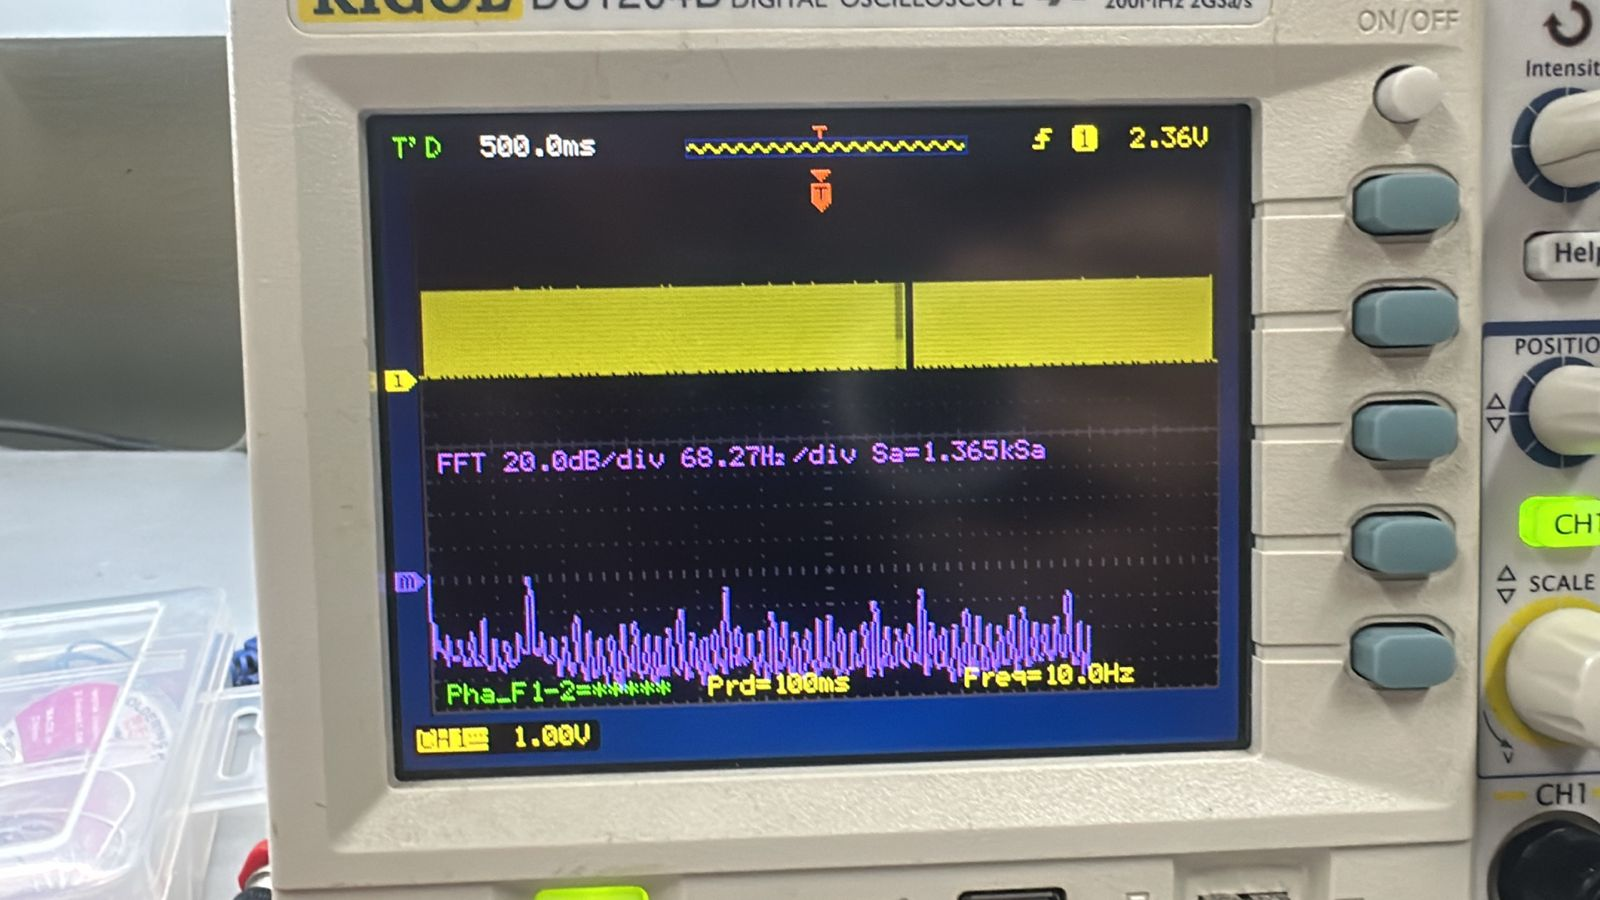
\includegraphics[width=0.5\textwidth]{img/entrada-100Hz.jpeg}
  \caption{Respuesta temporal y espectral de la señal cuadrada aplicada sobre la referencia del regulador para una frecuencia de $\SI{100}{\hertz}$.}
  \label{fig:entrada-100Hz}
\end{figure}

\begin{figure}[H]
  \centering
  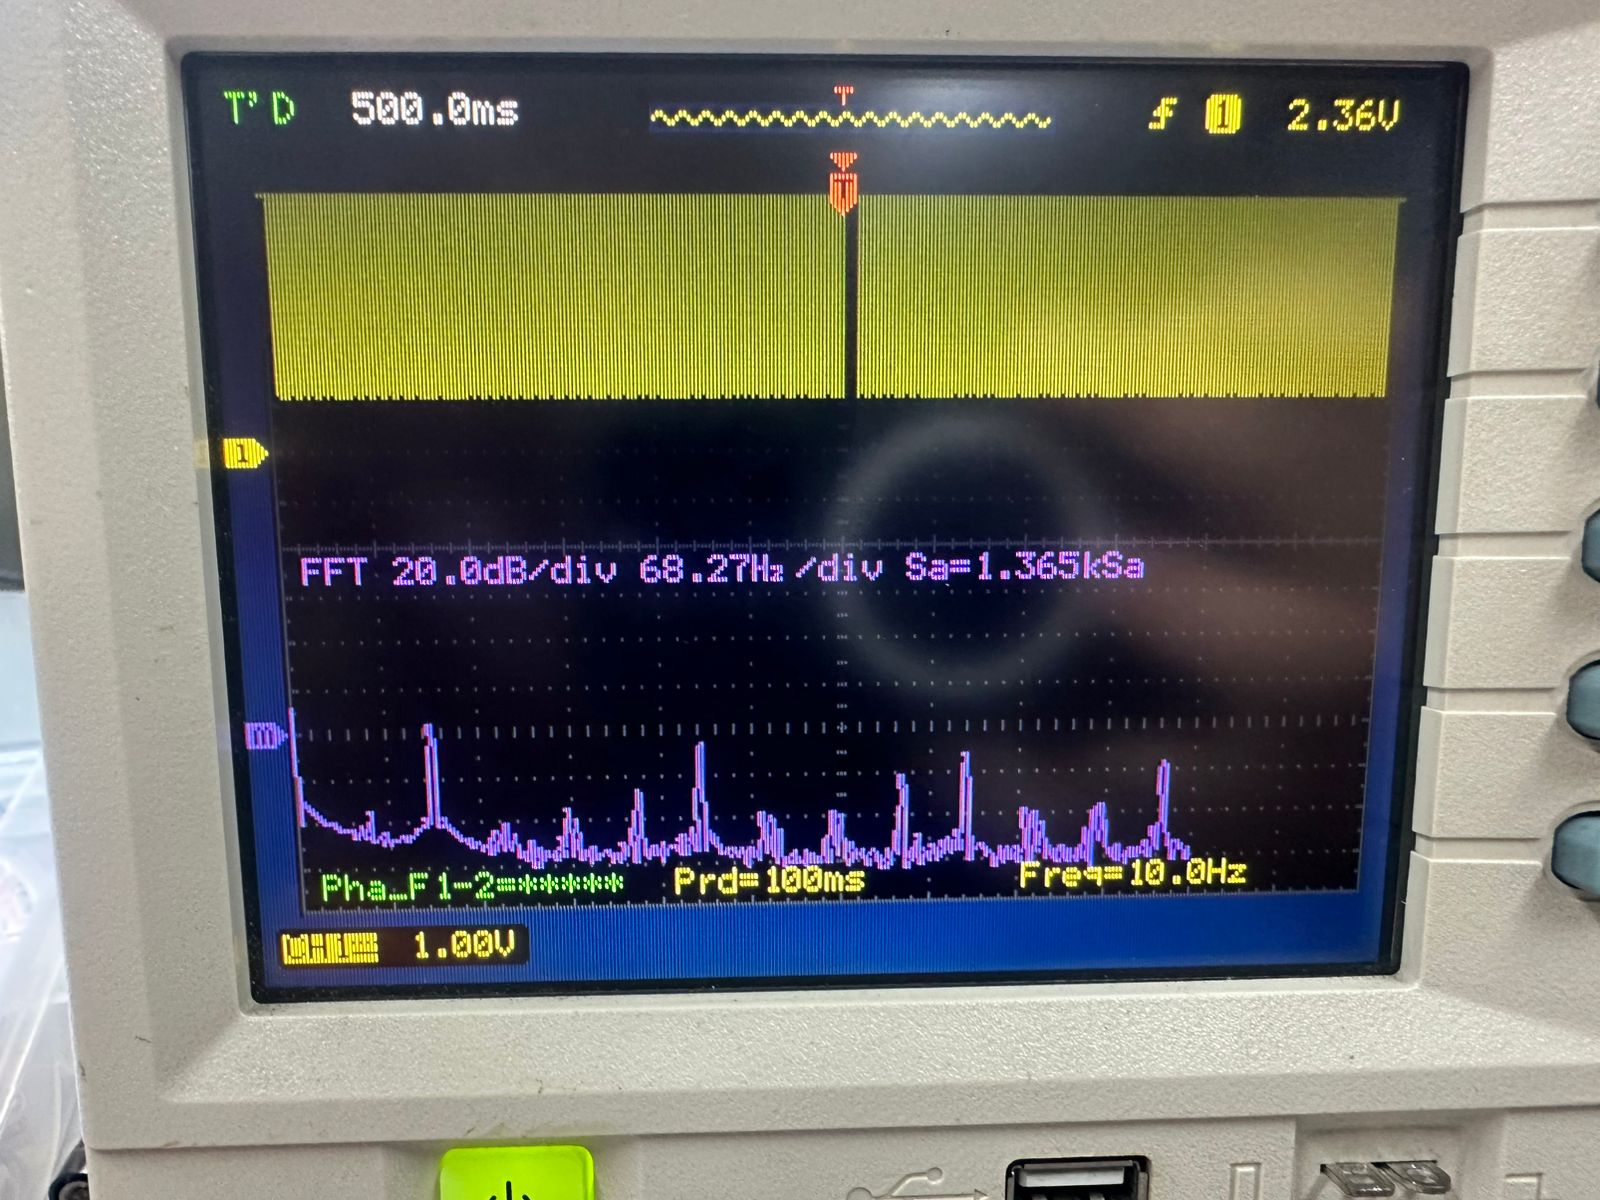
\includegraphics[width=0.5\textwidth]{img/salida-100Hz.jpeg}
  \caption{Respuesta temporal y espectral de la salida del regulador ante una excitación cuadrada de $\SI{100}{\hertz}$ aplicada sobre la referencia.}
  \label{fig:salida-100Hz}
\end{figure}

La presencia de estos componentes indica que el sistema comenzó a apartarse del comportamiento lineal ideal previsto para pequeñas señales. Este efecto puede atribuirse a limitaciones dinámicas del circuito al operar cerca de su frecuencia de corte, donde fenómenos asociados al ancho de banda finito del lazo, capacitancias internas, velocidad de respuesta del amplificador y no idealidades de la etapa de potencia comienzan a tener una influencia significativa sobre la forma de onda.

Como consecuencia, la reproducción de los armónicos deja de ser ideal y la señal de salida adquiere una forma más redondeada y distorsionada respecto de la cuadrada original.

\section{Resumen de resultados}

En la Tabla \ref{tab:resultados} se muestra un resumen de las mediciones efectuadas con sus resultados.

\begin{table}[H]
    \centering
    \begin{adjustbox}{width=\textwidth}
    \begin{tabular}{c c c c c c c}
    \noalign{\hrule height 1pt} % Línea más gruesa aquí
    Característica & Símbolo & Condiciones de prueba & Mín. & Típ. & Máx. & Unidad \\
    \hline
    Tensión de salida & $V_o$ & $0,1\,\text{A}\le I_o \le 1,5\,\text{A};~V_\text{REG} = 9,5\,\text{V}$ & 4,99 & 5,00 & 5,01 & V \\
    Eficiencia & $\eta$ & $I_o = 167\,\text{mA};~V_\text{REG} = 9,5\,\text{V}$ & - & 48,39 & - & \% \\
    Regulación de línea & $\mathrm{Reg_\text{lín}}$ & $0,25\,\text{V}\le V_\text{REG}\le 9,7\,\text{V};~I_o = 0,1\,\text{A}$ & - & 11,86 & - & mV/V \\
    Regulación de carga & $\mathrm{Reg_\text{car}}$ & $0\,\text{A}\le I_o \le 1,45\,\text{A}$ & - & 28,81 & - & m$\Omega$ \\
    Corriente límite & $I_\text{LÍM}$ & - & - & 1,45 & - & A \\
    Corriente de \textit{foldback} & $I_\text{FBK}$ & $V_o = 0\,$V & - & 450 & - & mA \\
    \noalign{\hrule height 1pt} % Línea más gruesa aquí
    \end{tabular}
    \end{adjustbox}
    \caption{Resumen de resultados.}
    \label{tab:resultados}
\end{table}

\section{Conclusiones}

A partir de las mediciones realizadas se concluye que el regulador implementado cumple satisfactoriamente con los objetivos principales de diseño, ya que mantiene una tensión de salida cercana al valor nominal, presenta una regulación de línea y de carga consistente con lo esperado y activa correctamente los mecanismos de limitación de corriente y protección \textit{foldback}. Al mismo tiempo, los ensayos dinámicos y de respuesta en frecuencia permitieron verificar que el lazo de tensión posee un comportamiento estable, aunque también pusieron en evidencia las limitaciones reales del prototipo al operar cerca del ancho de banda previsto. En conjunto, estos resultados validan la arquitectura adoptada y muestran que las diferencias observadas respecto de la simulación responden a no idealidades propias de los componentes y de la implementación física.

En cuanto a la impresión y el armado del PCB se concluye que es conveniente hacer pistas y \textit{pads} más anchos. Esto no solo simplifica la soldadura, sino que también hace más robusto al circuito y evita problemas como los cortocircuitos y los falsos contactos.

Como resultado importante de este \textit{checkpoint} se concluye que para futuros diseños deben tenerse en cuenta las específicaciones de los componentes usados, especialmente en lo relativo a sus tensiones y corrientes de salida. También se tendrá en cuenta que los modelos \texttt{Spice} de los mismos muchas veces son simplificados o incompletos. 

\section{Referencias}

[1] P. R. Gray, P. J. Hurst, S. H. Lewis y R. G. Meyer, \textit{Analysis and Design of Analog Integrated Circuits}. Hoboken, NJ: Wiley, 5ta ed., 2009.

[2] STMicroelectronics, ``TIP32C: Power transistor.'', 2006.

[3] Texas Instruments, ``TL431, TL432: Precision Programmable Reference.'', 2025.

[4] ON Semiconductor, ``BC556B, BC557A, B, C, BC558B: Amplifier transistors (PNP Silicon).'', 2007.

[5] Fairchild Semiconductor, ``BC547, BC547A, BC547B, BC547C: NPN General Purpose Amplifier.'', 1997.

[6] Semiconductores y Componentes, ``Disipadores.'', s.f.

[7] Texas Instruments, ``How to Properly Configure Unused Operational Amplifiers.'', SBOA204A, rev. Sept. 2018.

[8] Texas Instruments, ``LM158, LM258, LM2904, LM358: Industry-Standard Dual Operational Amplifiers.'', SLOS068AB, rev. Oct. 2024.

\end{document}